\chapter{Resultados}
\label{sec:results}

Essa seção apresenta os resultados das análises que desenvolvemos sobre os dados
da pesquisa OD 17. Começamos com a exploração dos recursos de visualização
suportados pelo \emph{CUBu}, com ênfase na codificação visual de atributos
densidade, distância e direção das viagens. Esses aspectos são apresentados a
seguir nas Seções~\ref{sec:density},~\ref{sec:trail-overlap},~\ref{sec:length-direction},~and~\ref{sec:coloring}.
Posteriormente, utilizando tais recursos visuais analisamos outros padrões de
mobilidade específicos a subconjuntos dos dados, os quais são detalhados nas
Seções~\ref{sec:strata},~\ref{sec:students},~\ref{sec:peak-hours},~\ref{sec:dist_reasons},~and~\ref{sec:mode}.

\section{Visualizando a densidade dos \emph{bundles}}
\label{sec:density}

Na Seção~\ref{sec:bundling} explicamos como a operação de \emph{bundling}
faz o agrupamento de trajetórias simplificando a visualização e reduzindo a oclusão
da imagem. No entanto, tal operação não nos diz quantas trajetórias foram agrupadas em
um \emph{bundle}. A solução para isso, primeiramente apresentada por \cite{holten06},
é desenhar linhas semi-transparentes, cada uma com uma transparência fixa $\alpha < 1$.
Assim, a combinação mostrará trajetórias de alta densidade como mais opacas e as de baixa
densidade como mais transparentes. Apesar da transparência ajudar na diferenciação
de áreas densas, ela por si só não é uma variável visual quantitativa forte \cite{slocum09}.
Então, codificamos também a densidade das trajetórias em cores, utilizando
os valores estimados pelo KDE durante o processo de \emph{bundling} (ver Seção~\ref{sec:bundling}).
A Figura~\ref{fig:bundled-graph-density}a mostra uma visualização obtida usando codificação
da densidade em cores aplicada em todo o conjunto de dados da OD17 contendo
as \num{685115} viagens. Podemos ver alguns caminhos com maior densidade, mas a imagem
ainda apresenta uma demasiada carga de informação e muitas áreas opacas. Isso ocorre pelo fato de que,
usualmente em GPUS de consumo comum, a transparência $\alpha$ é modelada por um valor
inteiro de 8 bits. Portanto, apenas 255 níveis de transparência diferentes são possíveis,
ou seja, apenas 255 níveis de densidade das trajetórias podem ser exibidos. Valores
de $\alpha$ muito altos saturam o canal de transparência
onde ocorrem as densidades mais altas - todas as densidades acima de 255 são fixadas
em 255. Valores abaixo de 1/255 resultam em nenhuma imagem, uma vez que
isso corresponde a opacidade zero na representação de 8 bits.

Para resolver este problema, mapeamos a densidade $\rho$ de duas maneiras,
transparência e cor. Já que $\rho$ é calculado precisamente como um número
de ponto flutuante durante a estimação do KDE, nenhum valor é truncado ou arredondado.
Essa estimativa da densidade permite modular a transparência para destacar ainda
mais as áreas de alta densidade e reduzir a oclusão da imagem -- uma outra alternativa
seria utilizar valores maiores de kernel $k$, o que agruparia ainda mais as trajetórias, gerando
\emph{bundles} mais fortes, porém também iria causar uma maior distorção das linhas.
A Figura~\ref{fig:bundled-graph-density}b mostra o \emph{bundling} aplicado nos mesmos
dados da Figura~\ref{fig:bundled-graph-density}a. Podemos observar que os \emph{bundles}
aparecem mais salientes após aplicar a modulação da transparência. A imagem sugere que a rede do tráfego metropolitano
pode ser dividida em algumas ramificações principais que são fortemente conectadas à área central,
onde a cidade de São Paulo está localizada. Isso faz sentido considerando que esta é a parte
mais populosa da área metropolitana. Além disso, a maioria dos sistemas de transporte
cruzam o centro da capital, incluindo linhas de metrô, trem, e as principais vias expressas.

\begin{figure}[!htb]
  \centering
  \captionsetup{justification=centering}
  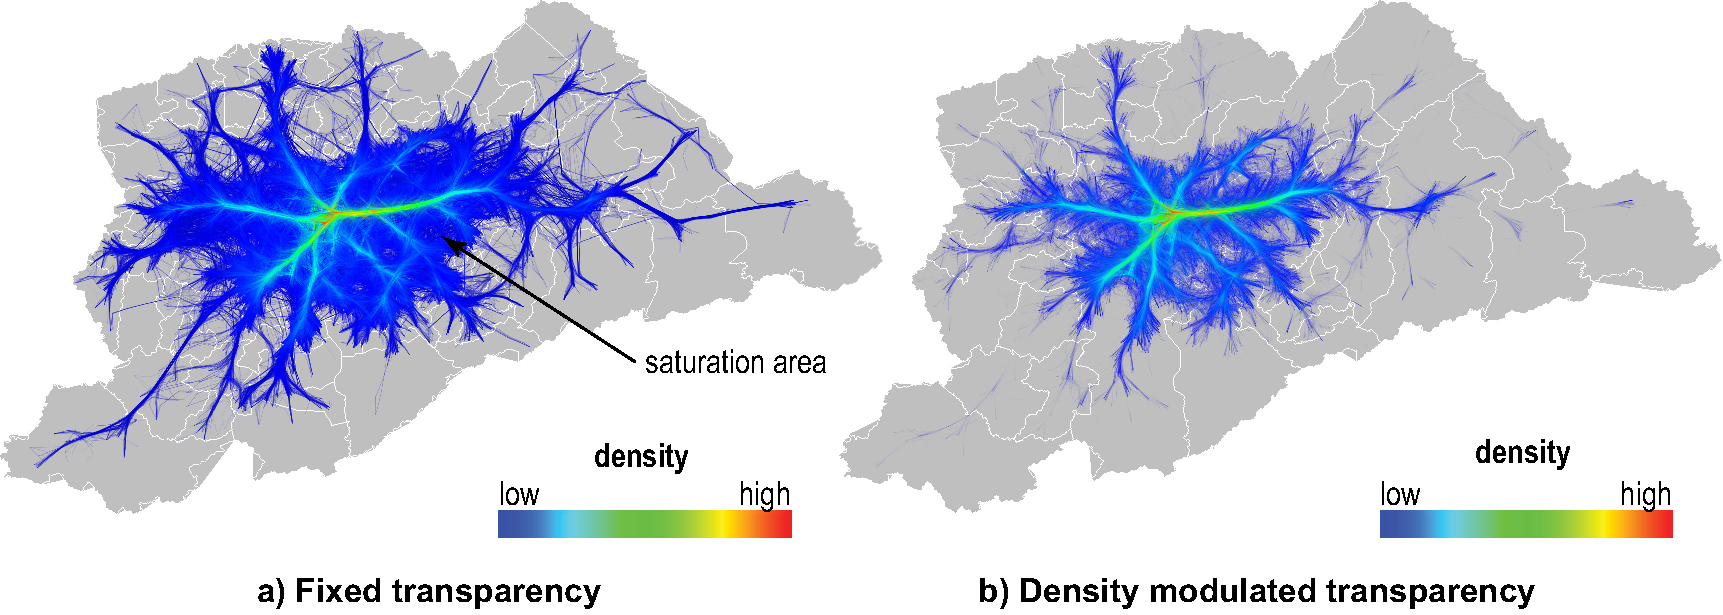
\includegraphics[width=0.98\textwidth]{../figuras/figure1}
  \caption{\emph{Bundling} das trajetórias coloridas pela densidade (a) valores fixos e \\(b) transparência modulada.}
  \label{fig:bundled-graph-density}  
\end{figure}

% % How we calculated 44%:
% %
% % 1. Take all trips that indicate bus, metro, and train as
% %    the main transportation mode -> this is the amount of
% %    trips by public transportation
% %
% % 2. Take all trips that indicate use of metro or train for
% %    some portion of the trip and divide that by the amount
% %    of trips by public transportation
% %
% % Using the tables from pages 46 and 49 of
% % http://www.metro.sp.gov.br/pesquisa-od/arquivos/Ebook%20Pesquisa%20OD%202017_final_240719_versao_4.pdf
% %
% % We consider that:
% % trips using bus as the main transportation mode: 8034
% % trips using train as the main transportation mode: 1245
% % trips using metro as the main transportation mode: 3400
% % total trips by public transportation: 8034 + 1245 + 3400 = 12679
% %
% % trips using metro for some portion of the trip: 3400
% % trips using train for some portion of the trip: 2272
% % total trips involving train or metro: 3400 + 2272 = 5672
% %
% % Percentage = 5672*100/12679 = 44.73%
% %
% % Not relevant for the text, just a curiosity:
% % the percentage in relation to all motorized trips is 5672*100/28280=20.05%

\section{Infraestrutura de metrô e trem \emph{vs} \emph{bundling}}
\label{sec:trail-overlap}

O sistema de transporte público é o mais utilizado pelos moradores da RMSP. O
impacto da malha ferroviária sobre o deslocamento de pessoas fica claro quando
desenhamos as linhas ferroviárias ao longo das trajetórias agrupadas com o
\emph{bundling}. A Figura~\ref{fig:rails} mostra a alta correspondência dos
\emph{bundles} com os caminhos das linhas ferroviárias (desenhadas em preto).
Tendo em vista que, de acordo com a pesquisa OD17, cerca de 44\% das viagens
diárias de transporte público envolvem metrô ou trens, este é um resultado
esperado. Curiosamente pode-se questionar se o sistema ferroviário foi planejado
com precisão para atender a demanda, como sugere a visualização agrupada, ou se
a disponibilidade dessa opção de transporte influenciou a existência de fluxos
tão densos. Embora não temos os insumos para responder a essa pergunta, os
gestores de tráfego podem usar esse tipo de visualização para elaborar políticas
para o transporte público. Apesar de não expressar nenhuma grande surpresa sobre os
dados analisados, este é um resultado bastante importante, pois consideramos que a alta
correlação entre o \emph{bundling} das trajetórias e as linhas das ferrovias
também indica boas configurações de parâmetros para esse tipo de visualização na
escala da região metropolitana.

Ressaltamos que que este tipo de correlação (de \emph{bundles} com estradas) não
é o mesmo que o utilizado no método RAEB, \cite{zeng:19}. No método RAEB, o
agrupamento foi feito explicitamente para seguir estradas. Em nosso caso, as
linhas são sobrepostas sobre \emph{bundles}, que foram gerados unicamente a partir dos
dados da OD. Pode-se argumentar que RAEB, neste sentido, produz \emph{bundles}
mais ``corretos'', uma vez que estes são forçados para seguir as estradas. No
entanto, olhando mais de perto, podemos ver que RAEB não pode ter todos os
\emph{bundles} seguindo precisamente todos os caminhos das estradas - pois isso
basicamente bloquearia qualquer agrupamento do \emph{bundling} e resultaria no próprio
mapa das estradas. Além disso, RAEB requer que o registro dos pontos das trajetórias
seja feito dentro de uma rede rodoviária precisa. Isso torna-o
significativamente mais complexo para implementar e mais caro para processar do
que nossa solução baseada em \emph{CUBu}.

\begin{figure}[!htb]
  \centering
  \captionsetup{justification=centering}
  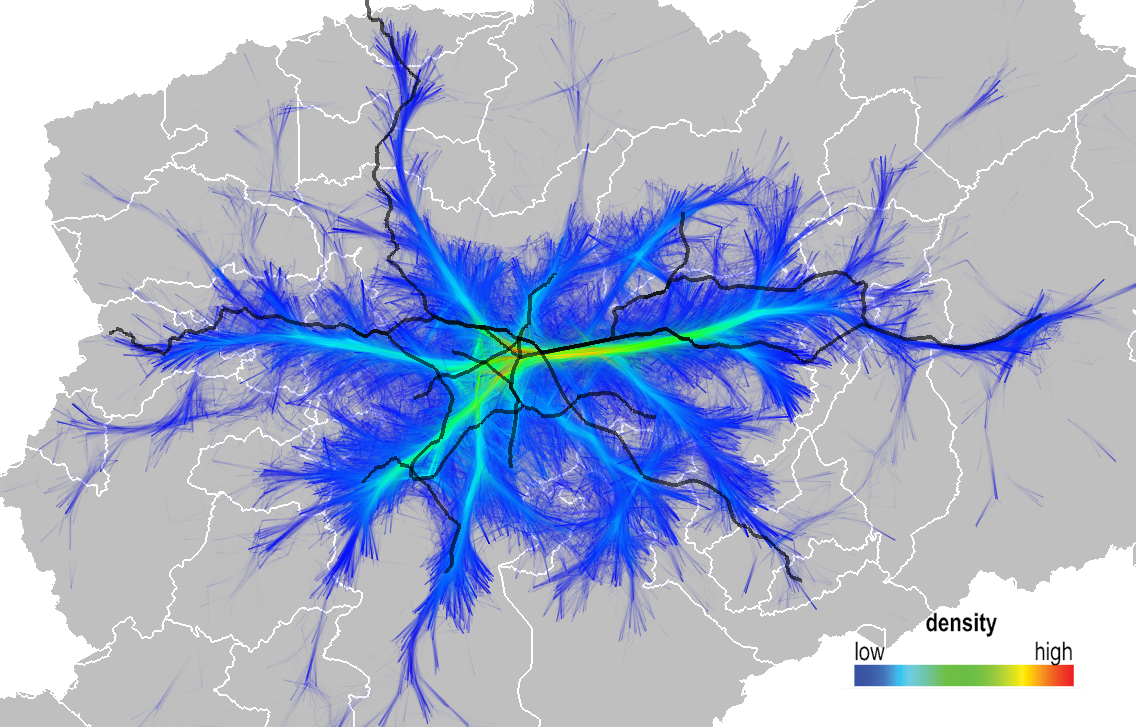
\includegraphics[width=0.98\textwidth]{../figuras/rail-lines.png}
    \caption{\emph{Bundling} das trajetórias coloridas pela densidade e a malha ferroviária da RMSP}
  \label{fig:rails}  
\end{figure}

\section{Mapeando distância e direção no \emph{bundling}}
\label{sec:length-direction}

Para explorar a mobilidade urbana por diferentes perspectivas, precisamos de
meios para visualizar os múltiplos atributos dos dados. Dois
importantes atributos para o estudo de padrões de mobilidade são distância
percorrida na viagem e a sua direção. As Figuras~\ref{fig:attributes-length} e
\ref{fig:attributes-direction} mostram a visualização de todo o conjunto de
dados OD17 mapeando a distância e direção, respectivamente.

Na Figura~\ref{fig:attributes-length} codificamos nas cores os comprimentos das
viagens. Nela utilizamos o mesmo mapa de cores (arco-íris) da
Figura~\ref{fig:rails}, além também de aplicar a modulação da transparência por densidade,
conforme explicado na Seção~\ref{sec:density}. Nesta imagem, podemos observar
uma única curva vermelha aparentemente na horizontal. Sua alta opacidade implica
que há muitas viagens longas, todas mapeadas perfeitamente para essa trajetória
entre a mesma origem e destino (se não o fizessem, veríamos um \emph{bundle} se
ramificando no formato de um leque em vez de uma curva precisa). Esta é uma
descoberta interessante que, argumentamos, não poderia ser facilmente encontrada
usando métodos não visuais. Apesar desse ponto fora do comum, as outras trajetórias,
em geral, percorrem distâncias regulares. \emph{Bundles} de longa distância como
este podem indicar falta de serviços ou recursos que não satisfazem as regiões
locais, obrigando as pessoas a percorrerem longas distâncias para acessá-los. A
pesquisa OD17 contém mais informações que podem ajudar a investigar o motivo
dessas longas viagens.

A Figura~\ref{fig:attributes-direction} mostra os mesmos dados da
Figura~\ref{fig:attributes-length}, mas ao invés da distância são as direções
das viagens que estão codificadas em cores. Para este atributo em específico,
usamos ainda um recurso do \emph{CUBu}, que separa trilhas em direções opostas
em dois \emph{bundles} quase paralelos. Podemos ver claramente a existência de
trajetórias paralelas ao longo dos \emph{bundles}, o que não é surpreendente
porque a pesquisa OD registra o trajeto típico das pessoas que inclui os
deslocamentos de ida e vinda de volta para suas origens. No entanto, essa
simetria das trajetórias possivelmente não seria observada se analisássemos um
curto período do dia.

\begin{figure}[!htb] \centering \captionsetup{justification=centering}
  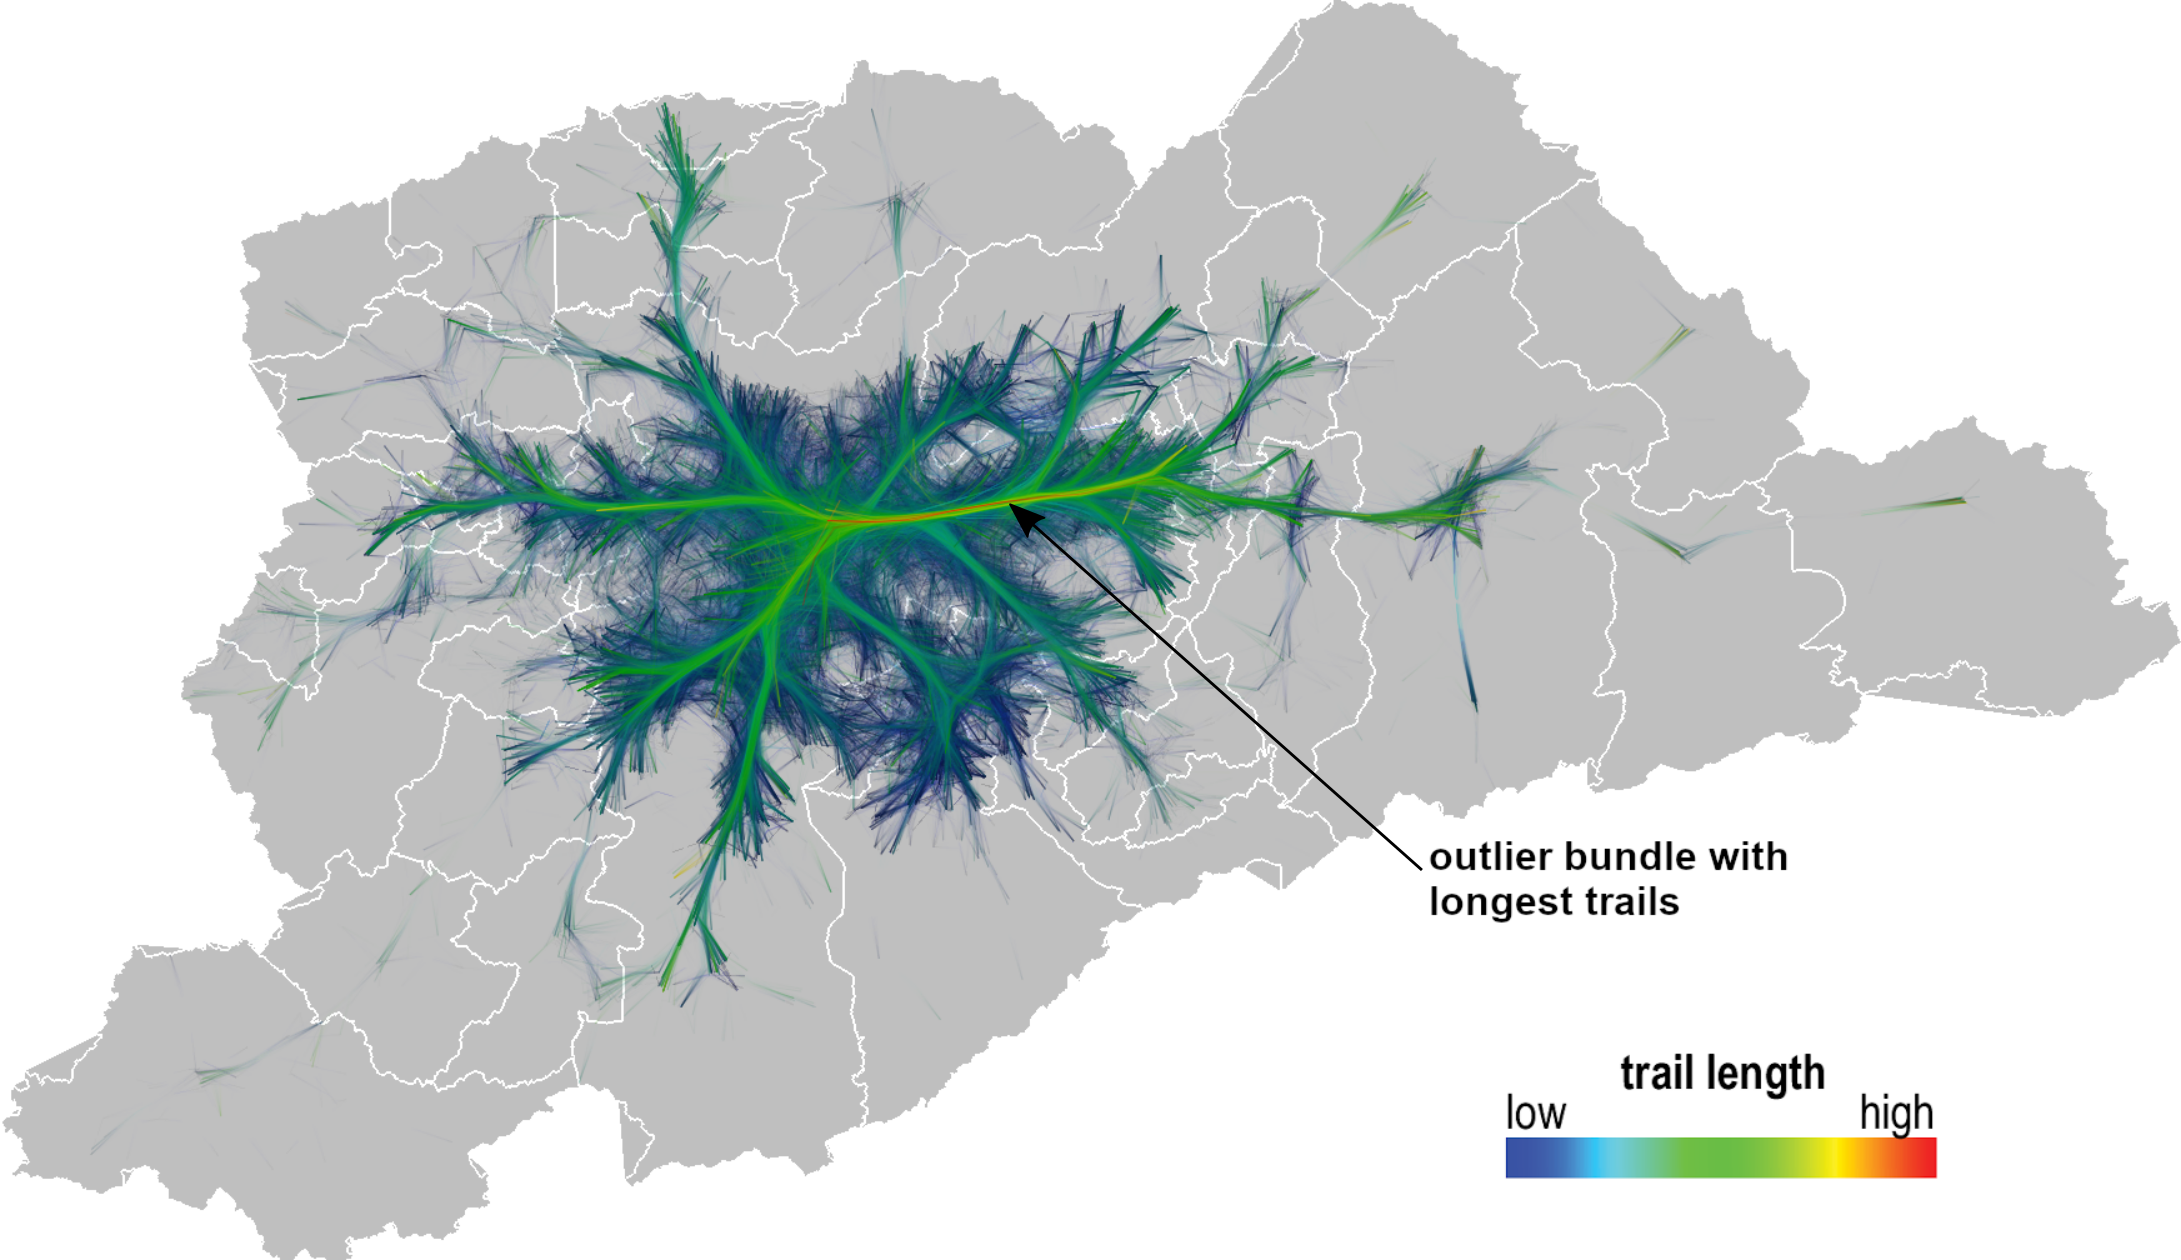
\includegraphics[width=0.98\textwidth]{../figuras/distances.png}
  \caption{Mapeamento da distância das viagens em cores. \label{fig:attributes-length}}
  \end{figure}

\begin{figure}[!htb]
  \centering
  \captionsetup{justification=centering}
  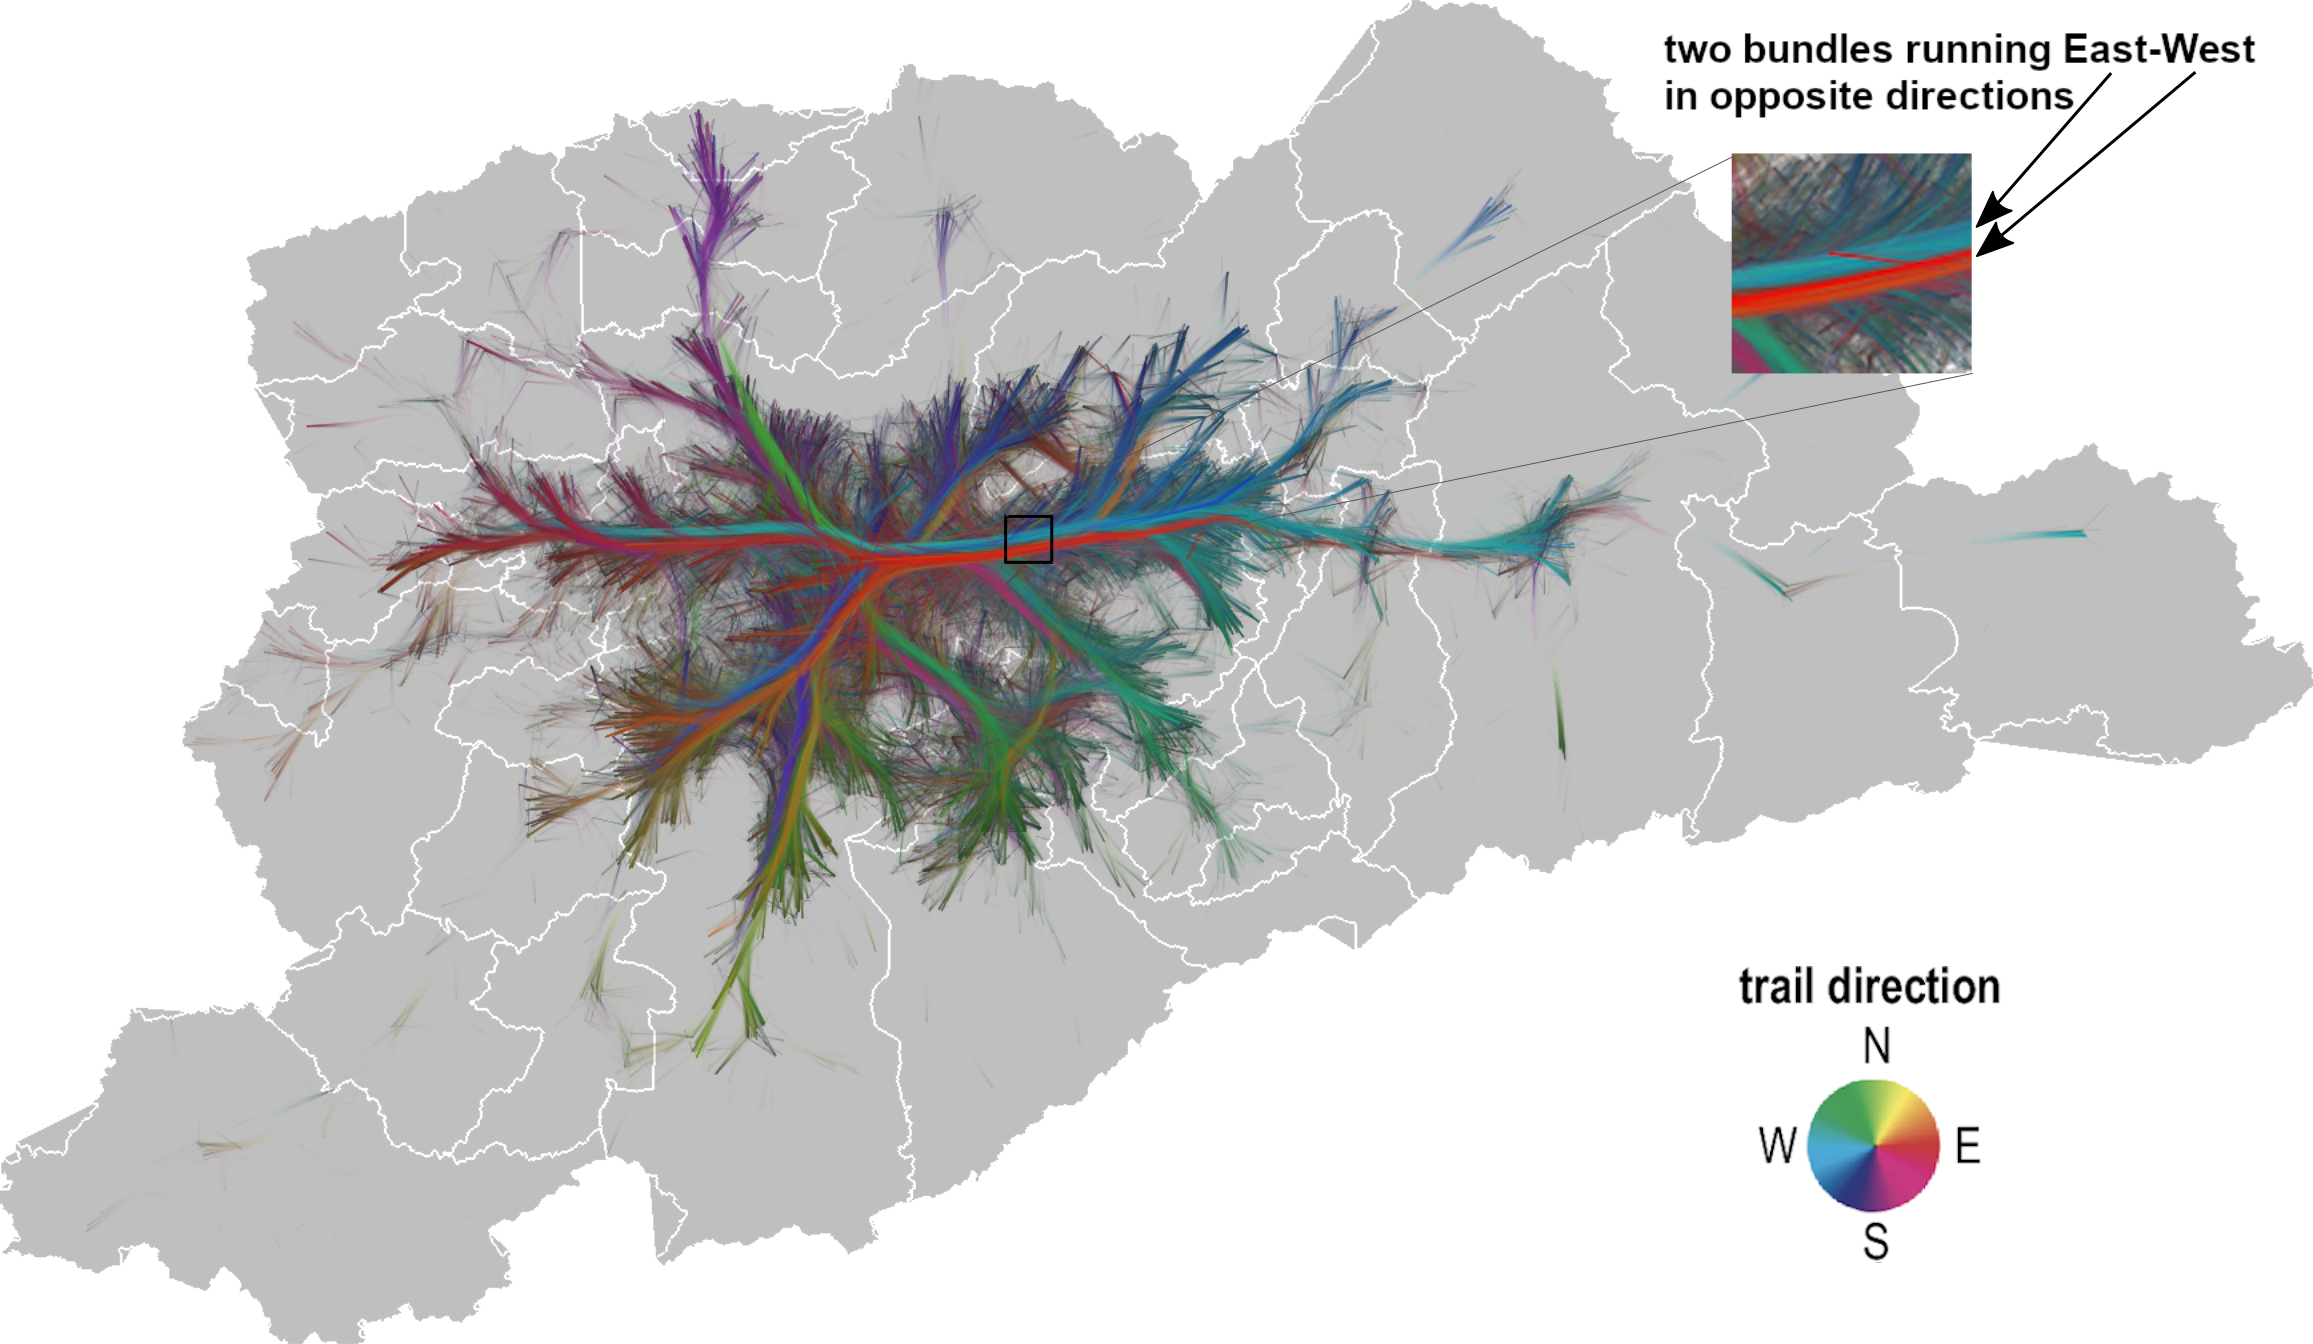
\includegraphics[width=0.98\textwidth]{../figuras/directions.png}
  \caption{Mapeamento da direção das viagens em cores. \label{fig:attributes-direction}}
\end{figure}

\section{Visualização dos modos de transporte: ônibus locais \emph{vs} intermunicipais}
\label{sec:coloring}

Como mostramos na Seção~\ref{sec:pesquisa-od}, o conjunto de dados OD17 contém
17 modos de transporte. Embora fosse ideal ser capaz de ver as 17 categorias ao
mesmo tempo em nossa visualização com \emph{bundling}, isso não seria fácil de
se obter, uma vez que exigiria a codificação simultânea de 17 diferentes
categorias de transporte. Então, nós utilizamos a transparência para esconder
trajetórias de acordo com seletores que podem ser configurados na interface para
filtrar as trajetórias pelo modo de transporte. A
Figura~\ref{fig:bus-integration} mostra como nos aplicamos tais filtros para
visualizar a integração entre os ônibus da cidade de São Paulo (ônibus locais) e
os ônibus intermunicipais. As trajetórias originais e agrupadas com \emph{bundling}
são apresentadas lado a lado. Cada meio de transporte tem uma coloração distinta -
oliva para ônibus locais e azul para ônibus intermunicipais.

Podemos ver mais claramente na Figura~\ref{fig:bus-integration-zoom} que esses diferentes sistemas
de transporte parecem se complementar. A cidade de São Paulo tem um comércio e
uma indústria muito ativa, que recebe muitos trabalhadores advindos das cidades
vizinhas. Assim, a disponibilidade de transporte público e sua integração é
muito importante para essas pessoas. Esse tipo de filtragem juntamente com as
técnicas de \emph{bundling} ajudam a entender melhor as correlações entre os
atributos dos dados - neste caso, modos de transporte.

\begin{figure}[!htb]
  %\centering
  %\raggedright\noindent\hspace{-\margemesq}\hspace{.01\paperwidth}%
  %\begin{subfigure}{0.49\paperwidth}
  \raggedright\noindent\hspace{-.02\textwidth}%
  \begin{subfigure}{0.55\textwidth}
    \centering
    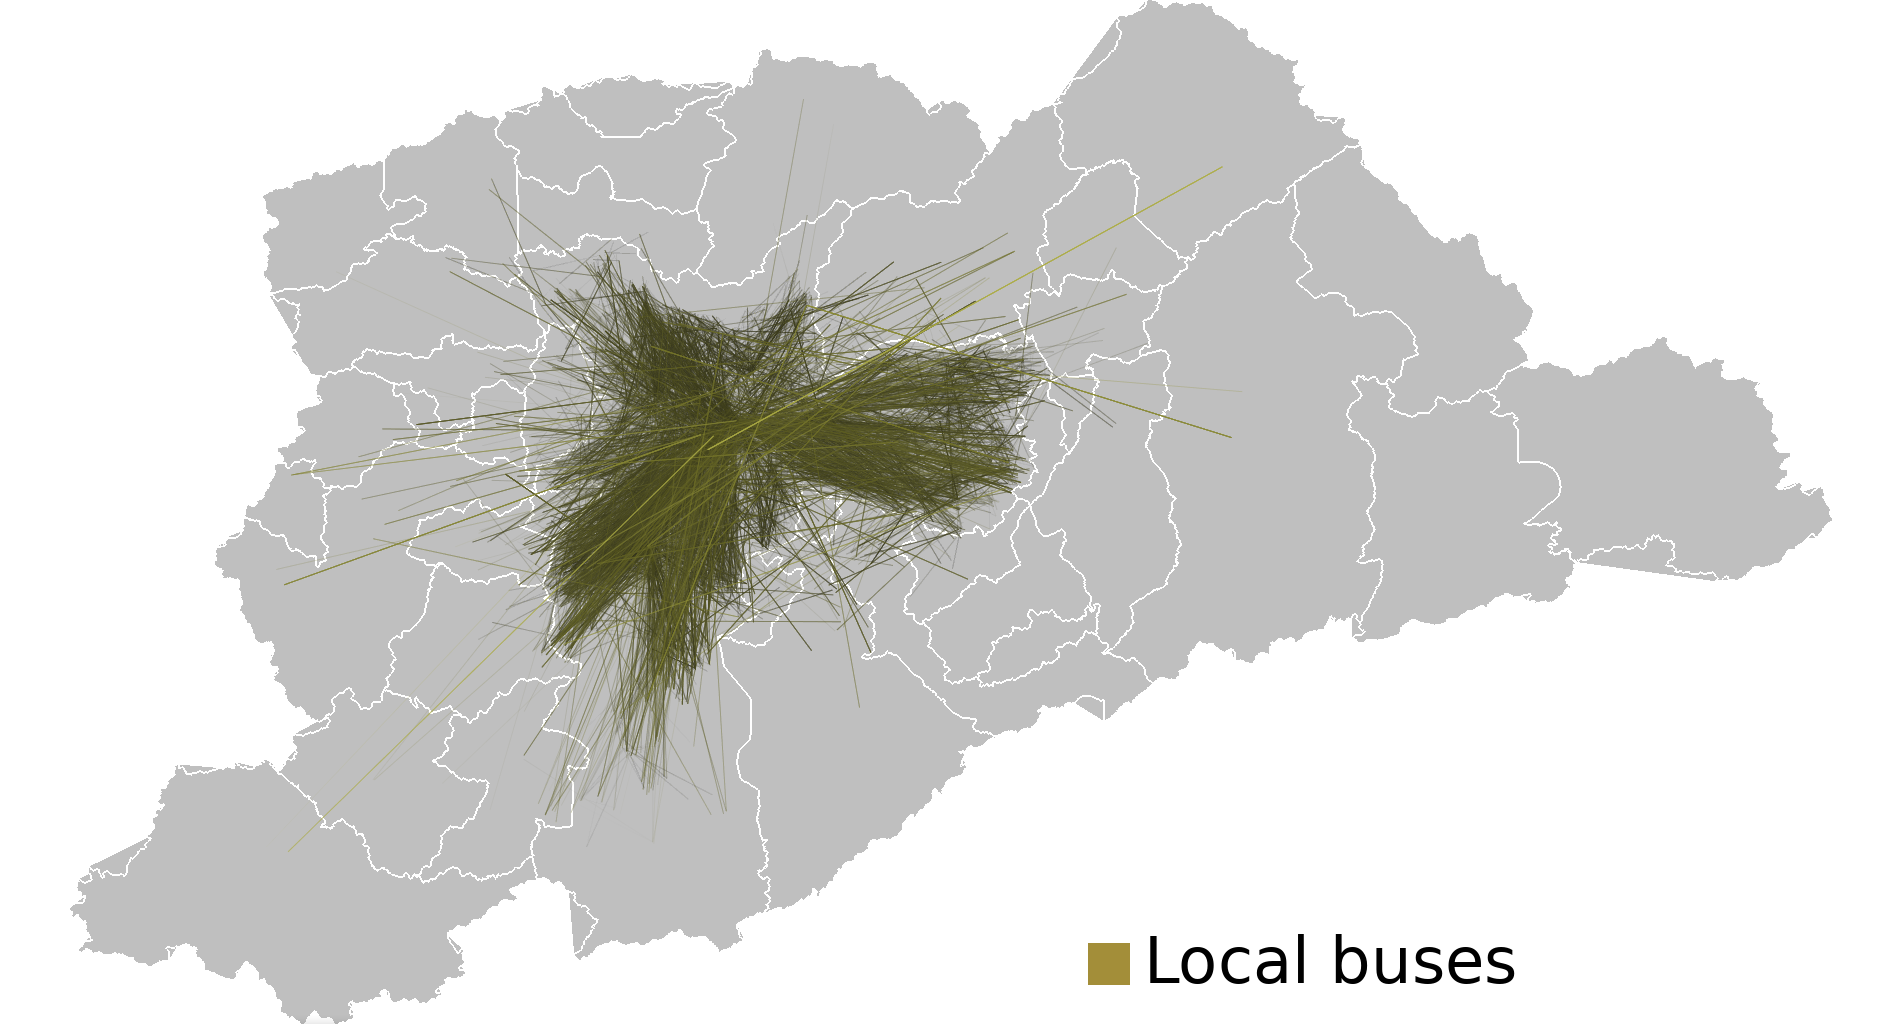
\includegraphics[width=1\textwidth]{../figuras/busesLocalXmetropolitan/unbundled-buses.png}
    \caption{\label{fig:bus-integration-a}}
  \end{subfigure}\nobreak%
  %\begin{subfigure}{0.49\paperwidth}
  \hspace{-.06\textwidth}\nobreak%
  \begin{subfigure}{0.55\textwidth}
    \centering
    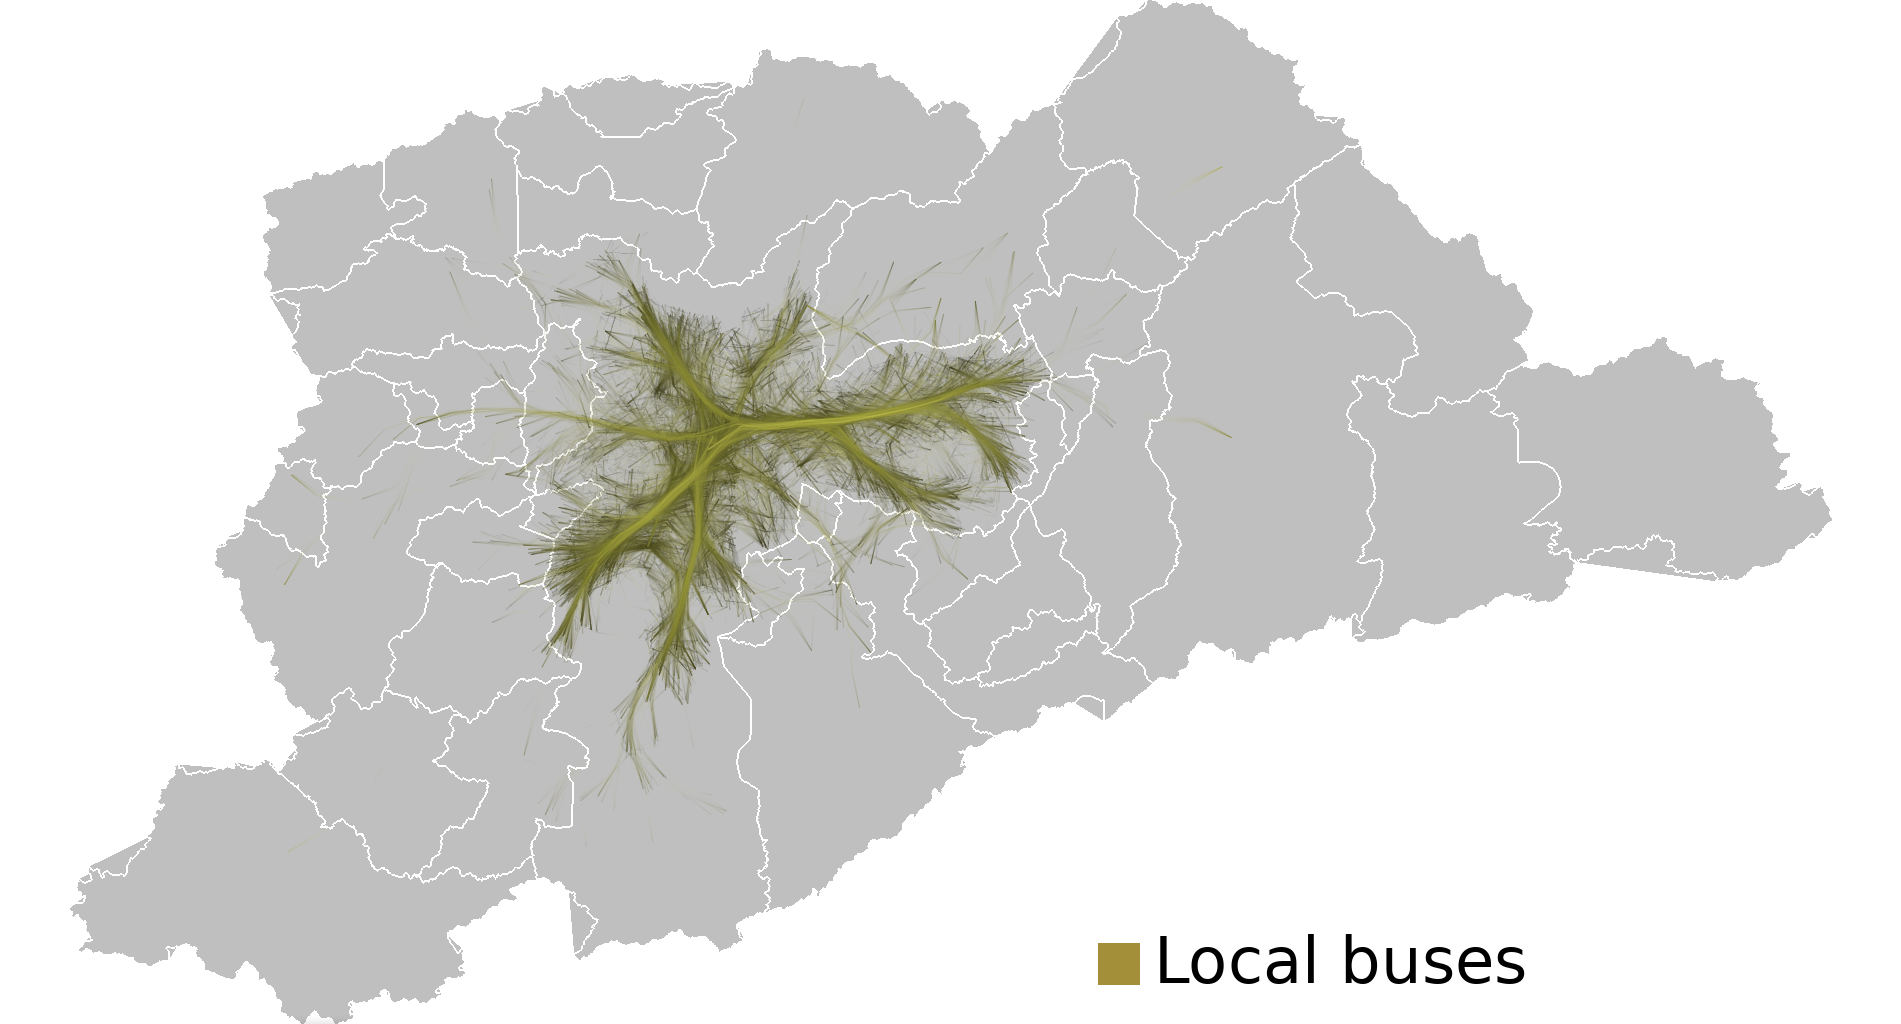
\includegraphics[width=1\textwidth]{../figuras/busesLocalXmetropolitan/bundled-buses-length.png}
    \caption{\label{fig:bus-integration-b}}
  \end{subfigure}

  %\noindent\hspace{-\margemesq}\hspace{.01\paperwidth}\begin{subfigure}{0.49\paperwidth}
  \raggedright\noindent\hspace{-.02\textwidth}%
  \begin{subfigure}{0.55\textwidth}
    \centering
    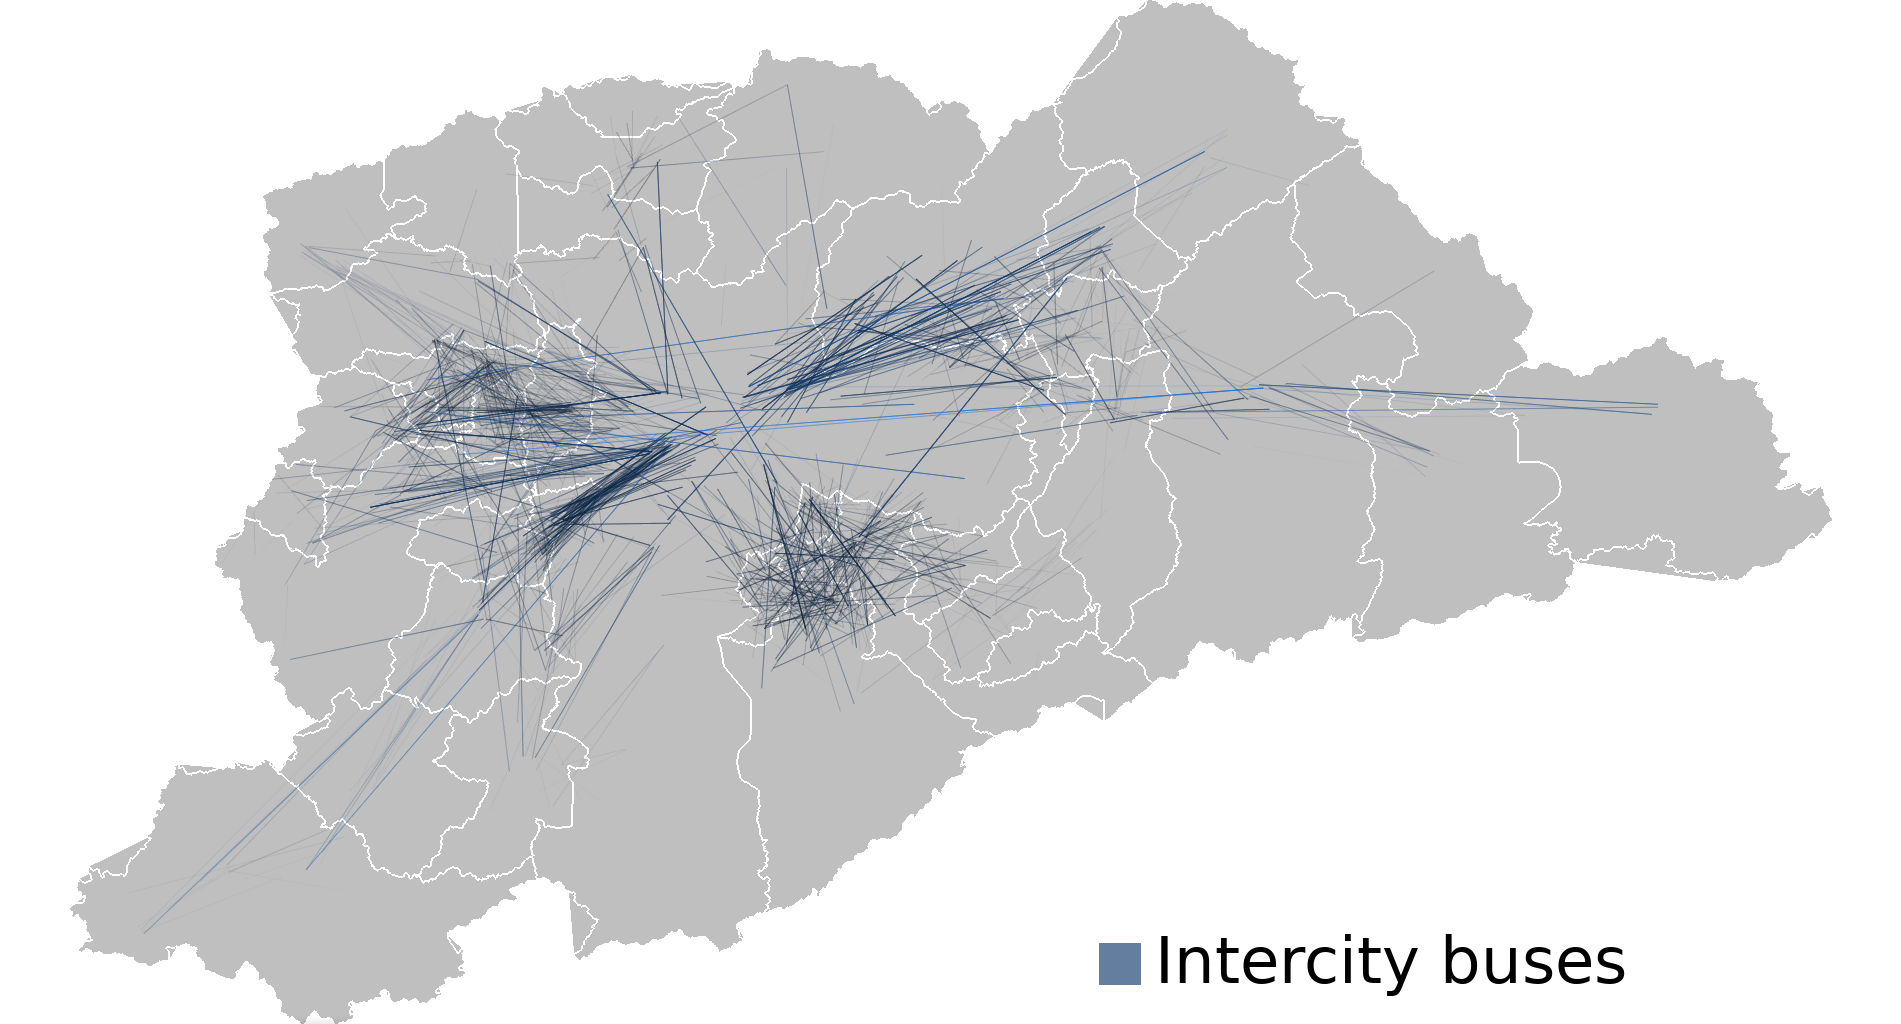
\includegraphics[width=1\textwidth]{../figuras/busesLocalXmetropolitan/unbundled-metropolitan-buses.png}
    \caption{\label{fig:bus-integration-c}}
  \end{subfigure}\nobreak%
  \hspace{-.06\textwidth}\nobreak%
  \begin{subfigure}{0.55\textwidth}
  %\begin{subfigure}{0.49\paperwidth}
    \centering
    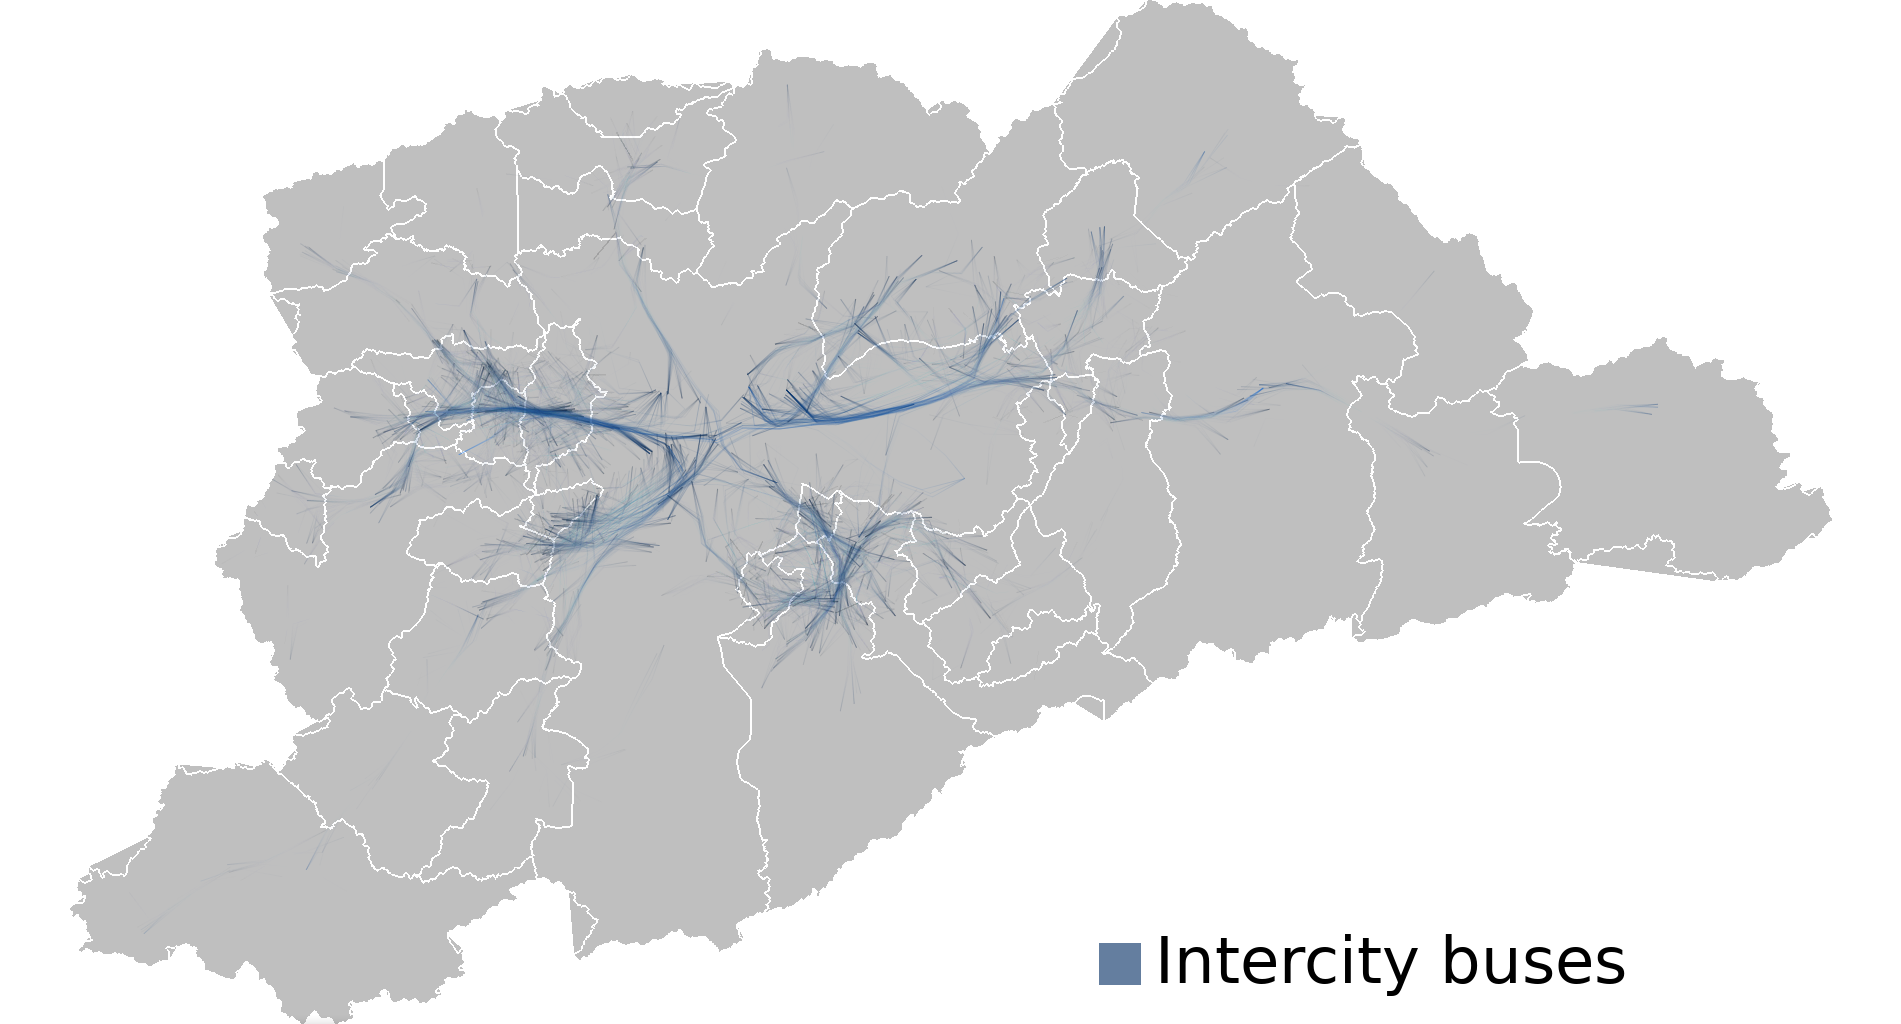
\includegraphics[width=1\textwidth]{../figuras/busesLocalXmetropolitan/bundled-metropolitan-buses-length.png}
    \caption{ \label{fig:bus-integration-d}}
  \end{subfigure}

  %\noindent\hspace{-\margemesq}\hspace{.01\paperwidth}\begin{subfigure}{0.49\paperwidth}
  \raggedright\noindent\hspace{-.02\textwidth}%
  \begin{subfigure}{0.55\textwidth}
    \centering
    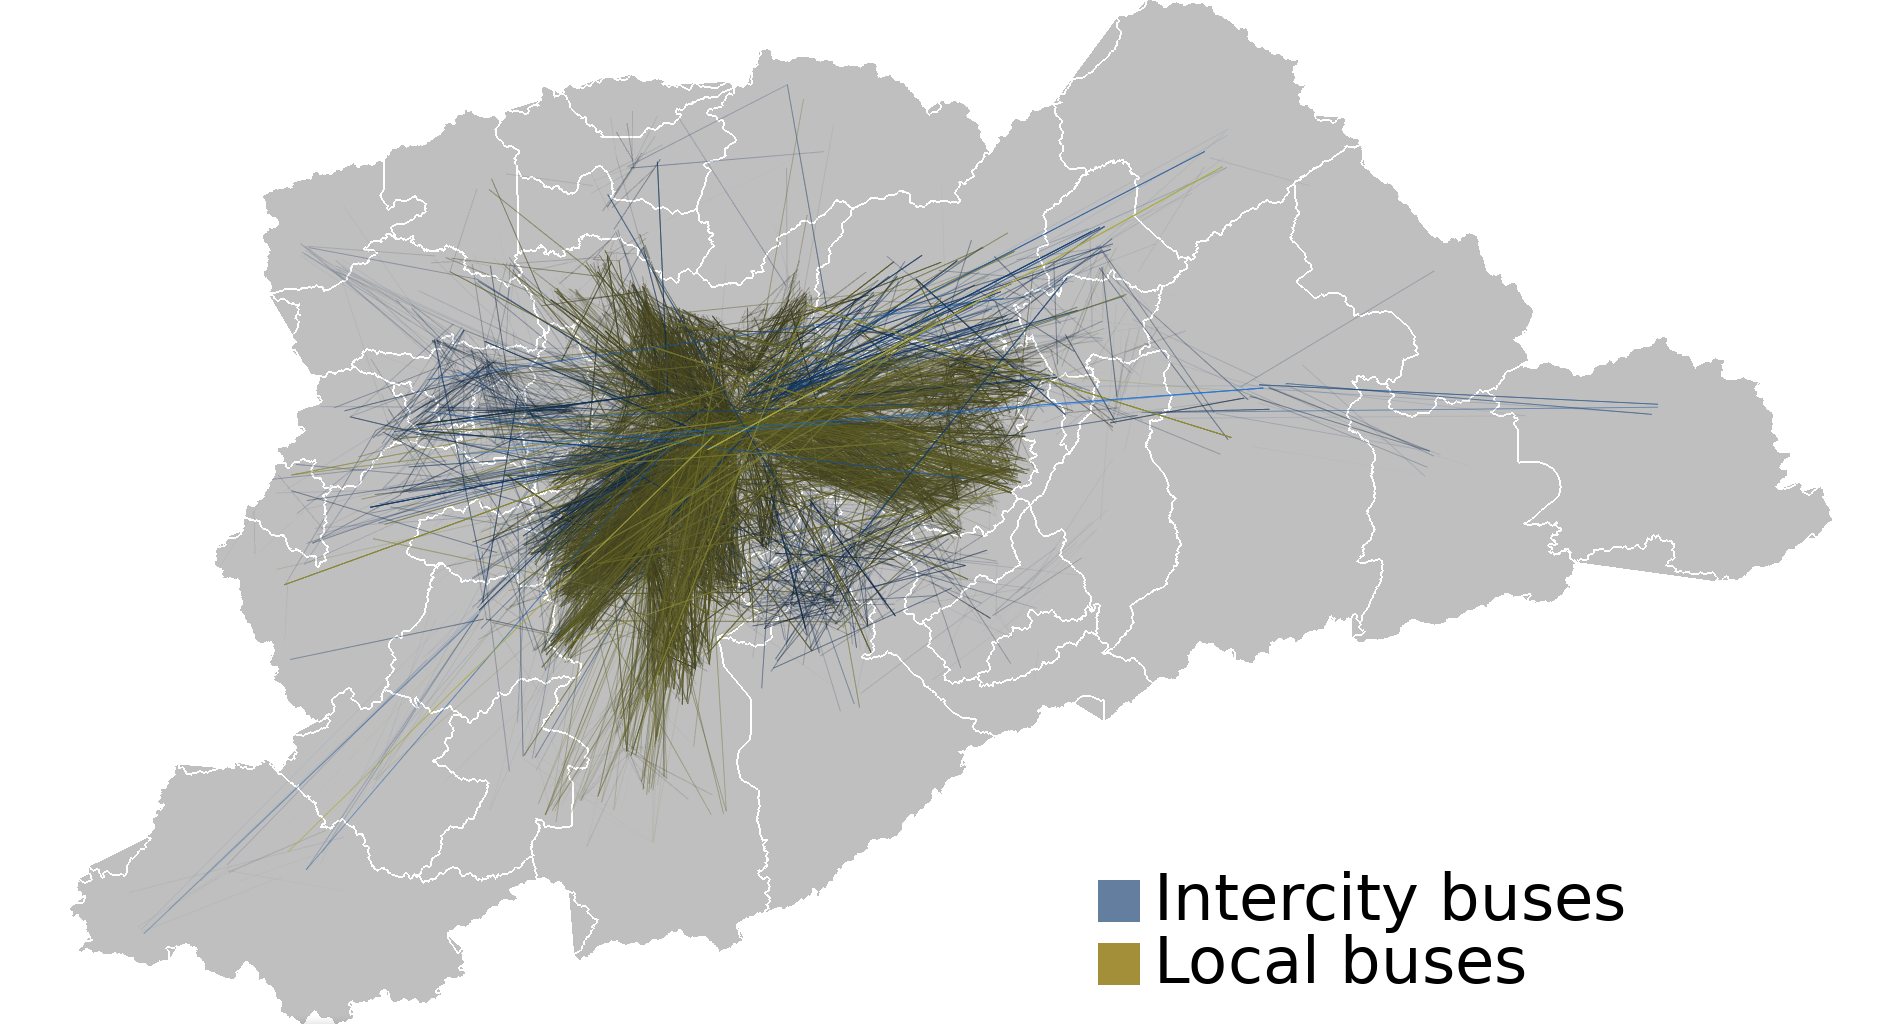
\includegraphics[width=1\textwidth]{../figuras/busesLocalXmetropolitan/unbundled-buses-and-metropolitan.png}
    \caption{\label{fig:bus-integration-e}}
  \end{subfigure}\nobreak%
  \hspace{-.06\textwidth}\nobreak%
  \begin{subfigure}{0.55\textwidth}
  %\begin{subfigure}{0.49\paperwidth}
    \centering
    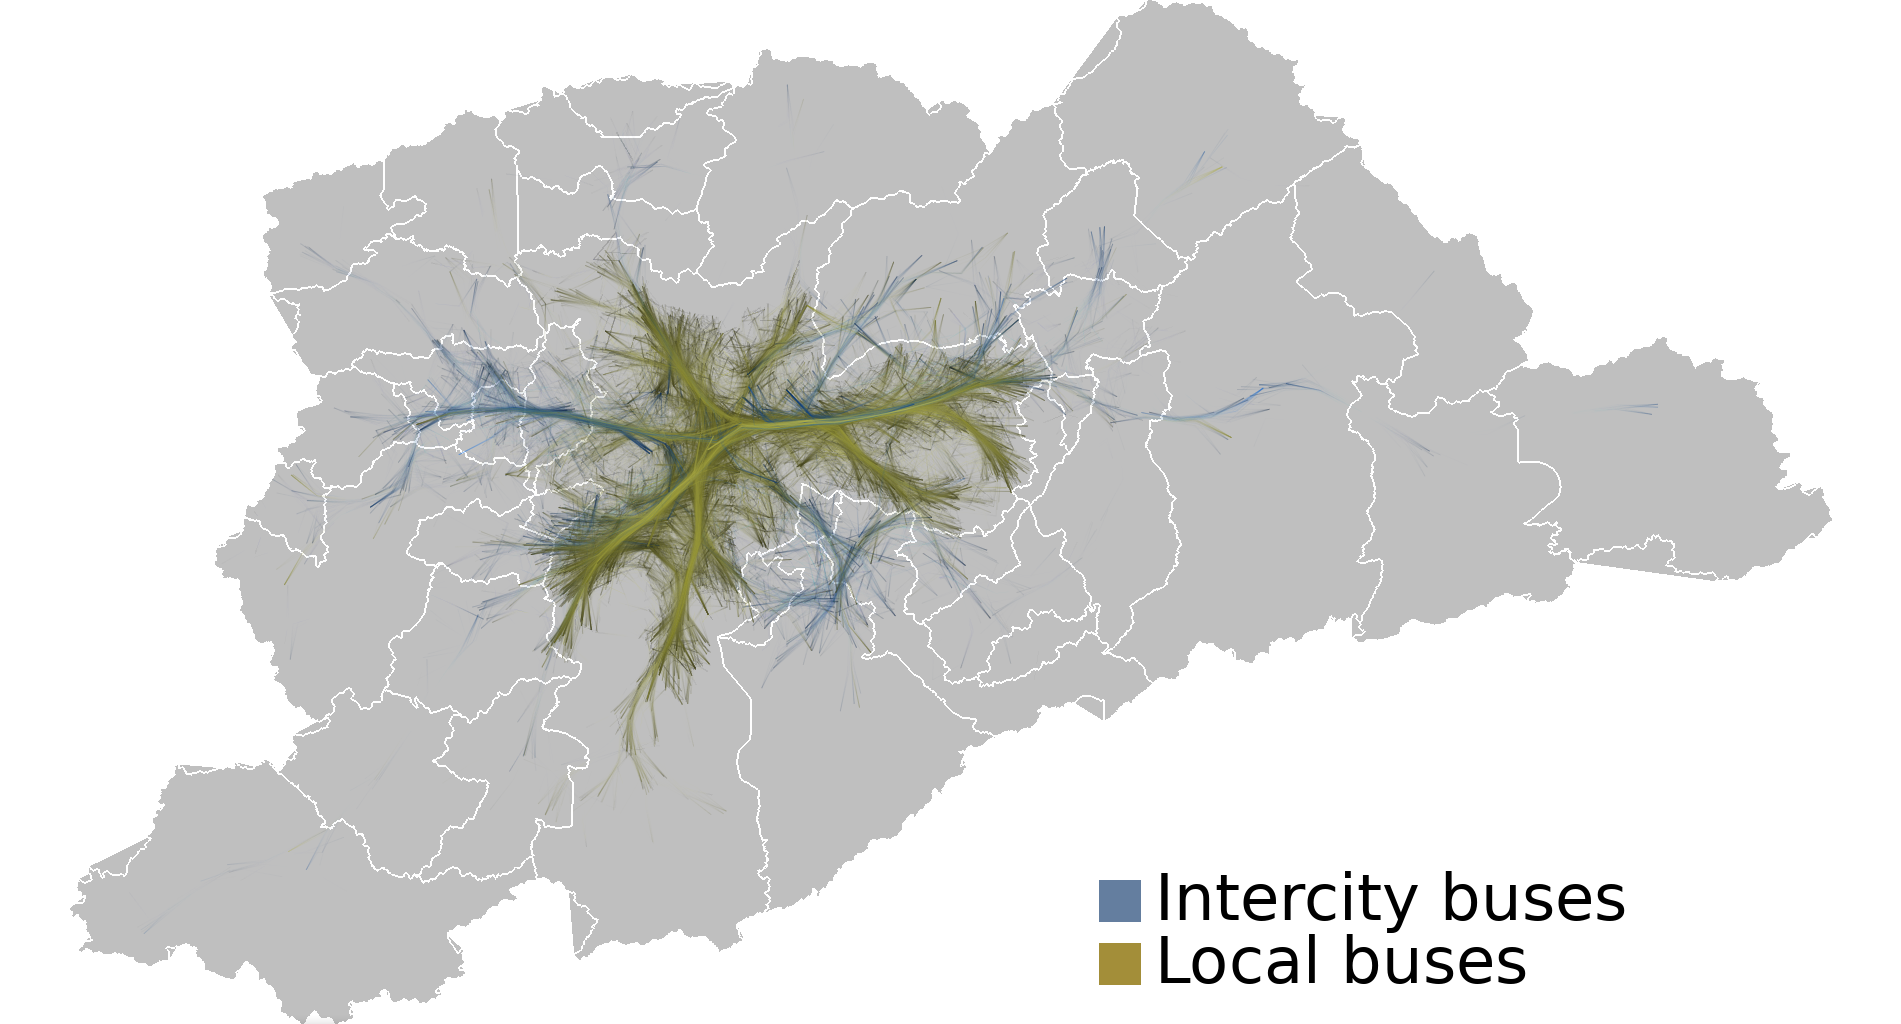
\includegraphics[width=1\textwidth]{../figuras/busesLocalXmetropolitan/bundled-buses-and-metropolitan-length.png}
    \caption{\label{fig:bus-integration-f}}
  \end{subfigure}
  \caption{Viagens filtradas pelo modo de transporte: ônibus locais e intermunicipais. Dados originais à esquerda (a, c, e)  e \emph{bundling} à direita (b, d, f). \label{fig:bus-integration}}
\end{figure}

\begin{figure}[!htb]
  \centering
  \captionsetup{justification=centering}
  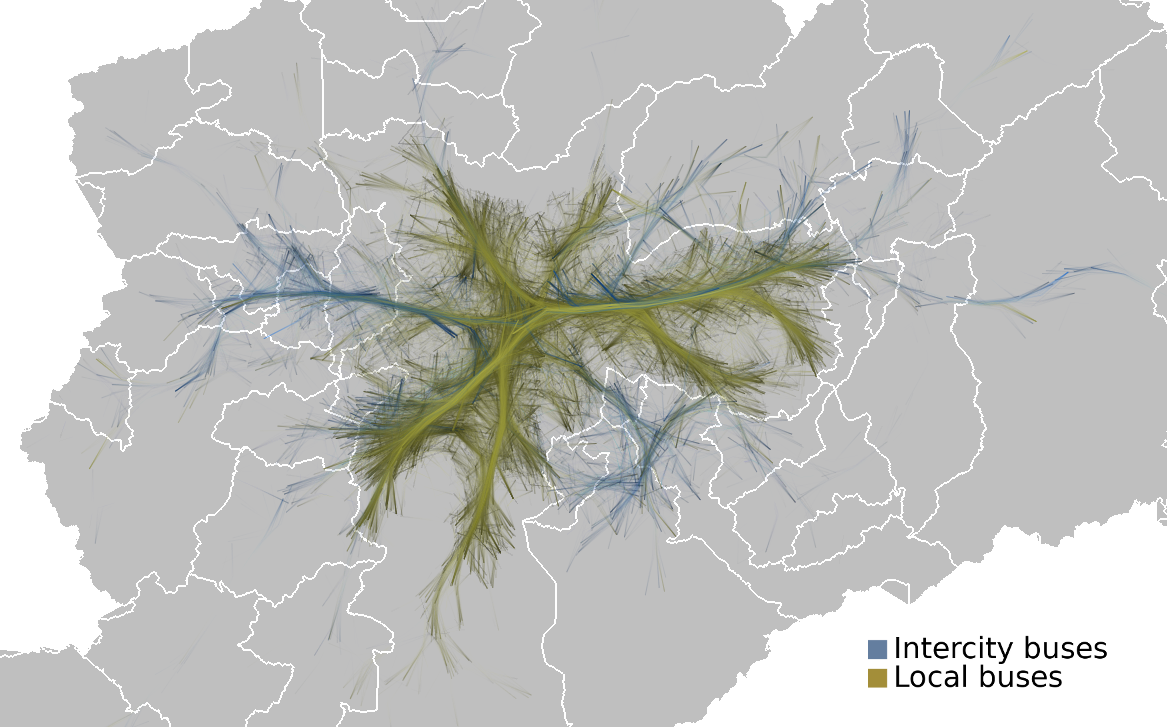
\includegraphics[width=0.98\textwidth]{../figuras/local-intercity-buses}
  \caption{Viagens filtradas pelo modo de transporte: ônibus locais e intermunicipais (ZOOM). \label{fig:bus-integration-zoom}}
\end{figure}

\section{Visualização das diferentes classes sociais}
\label{sec:strata}

% We used our bundle
% visualization to study how citizens with different economical conditions
% commute in the SPMA. The Brazilian Economical Classification Criterion
% (BECC)\,\cite{cceb2008} is the official social-economic index used in the
% Brazilian Demographic Census, which is performed by the Brazilian Institute of
% Geography and Statistics. It measures the purchasing power of the Brazilian
% society. The BECC is divided into six levels or strata (Table~\ref{tab:becc}).
% This index is used in the OD17 survey to complement the mobility data.
% Table~\ref{tab:becc} also shows the average monthly income in the local
% currency (Brazilian reals) and in US dollars, and the number of trips in the
% SPMA for each BECC level considering the whole population and only citizens
% with age between 6 and 18 years that commute for study (see
% Section~\ref{sec:students}).

Usamos nossa visualização com \emph{bundling} para estudar como os cidadãos com diferentes
condições econômicas se deslocam na RMSP. O Critério de Classificação Econômica
Brasileira (CCEB), \cite{cceb2008} é o índice socioeconômico oficial utilizado no Censo
Demográfico Brasileiro, realizado pelo Instituto Brasileiro de Geografia e
Estatística (IBGE). Ele mede o poder de compra da sociedade brasileira. O CCEB é
dividido em seis níveis ou estratos (Tabela~\ref{tab:becc}). Este índice é usado na pesquisa
OD17 para complementar os dados de mobilidade. A Tabela~\ref{tab:becc} também mostra a renda
média mensal (em reais), e o número de viagens na RMSP para cada nível do CCEB considerando toda a população e apenas
os cidadãos com idade entre 6 e 18 anos que se deslocam para fins de estudos (consulte a
Seção~\ref{sec:students}).

\begin{table}[!htb]
  \small
  \newcommand{\hdr}[1]{\bfseries#1}
  \centering
  \caption{Viagens agrupadas pelo índice CCEB income level, social stratum, and traveler age.\label{tab:becc}}
  \begin{tabular}{>{\footnotesize}c>{\footnotesize}r>{\footnotesize}r>{\footnotesize}r>{\footnotesize}r}
    \toprule
    \multirow{2}[2]{*}{\hdr{Nível CCEB}} & \hdr{Renda mensal} & \hdr{Viagens} & \hdr{Viagens de estudantes}\\
    & \hdr{em reais (R\$)} & \hdr{totais} & \hdr{entre 6 e 18 anos}\\
    \midrule
    A   & 23,345    & 3,062,892  &   184,772\\
    B1  & 10,386    & 3,854,040  &   260,652\\
    B2  & 5,363     & 12,856,182 &   963,242\\
    C1  & 2,965     & 11,277,159 &   976,745\\
    C2  & 1,691     & 7,852,806  &   721,218\\
    D-E & 708       & 2,233,801  &   219,612\\
    \bottomrule
  \end{tabular}
\end{table}

Para comparar os padrões de mobilidade de diferentes estratos sociais CCEB,
aplicamos \emph{bundling} nas viagens de cada estrato separadamente, como
mostrado nas Figuras~\ref{fig:becc-axd-e}~até~\ref{fig:becc-d-e}. Observamos
diferenças significativas nos padrões de mobilidade entre os níveis de renda
mais altos e mais baixos, como mostra a Figura~\ref{fig:becc-axd-e}. O nível $A$
Figuras~\ref{fig:becc-a} apresenta alta densidade no centro da RMSP, que inclui
o entorno do centro da capital. A maior densidade está localizada nos bairros
oeste, sudoeste e nordeste próximos ao centro. Existem fluxos de densidade entre
a capital e as cidades de Barueri e Cotia, que possuem áreas residenciais de
alta renda. Existem outros fluxos de alta densidade ligando a capital às cidades
de São Bernardo do Campo e Santo André. Comparando A ao nível D-E (Figura 18),
vemos que D-E tem os fluxos densos mais elevados na região leste da capital. No
mapa de níveis D-E, podemos ver a ausência de fluxos de alta densidade nas
regiões mais próximas do centro da capital; em contraste, eles estão presentes
no mapa de nível A.

\begin{figure}[!htb]
  \centering
  \captionsetup{justification=centering}
  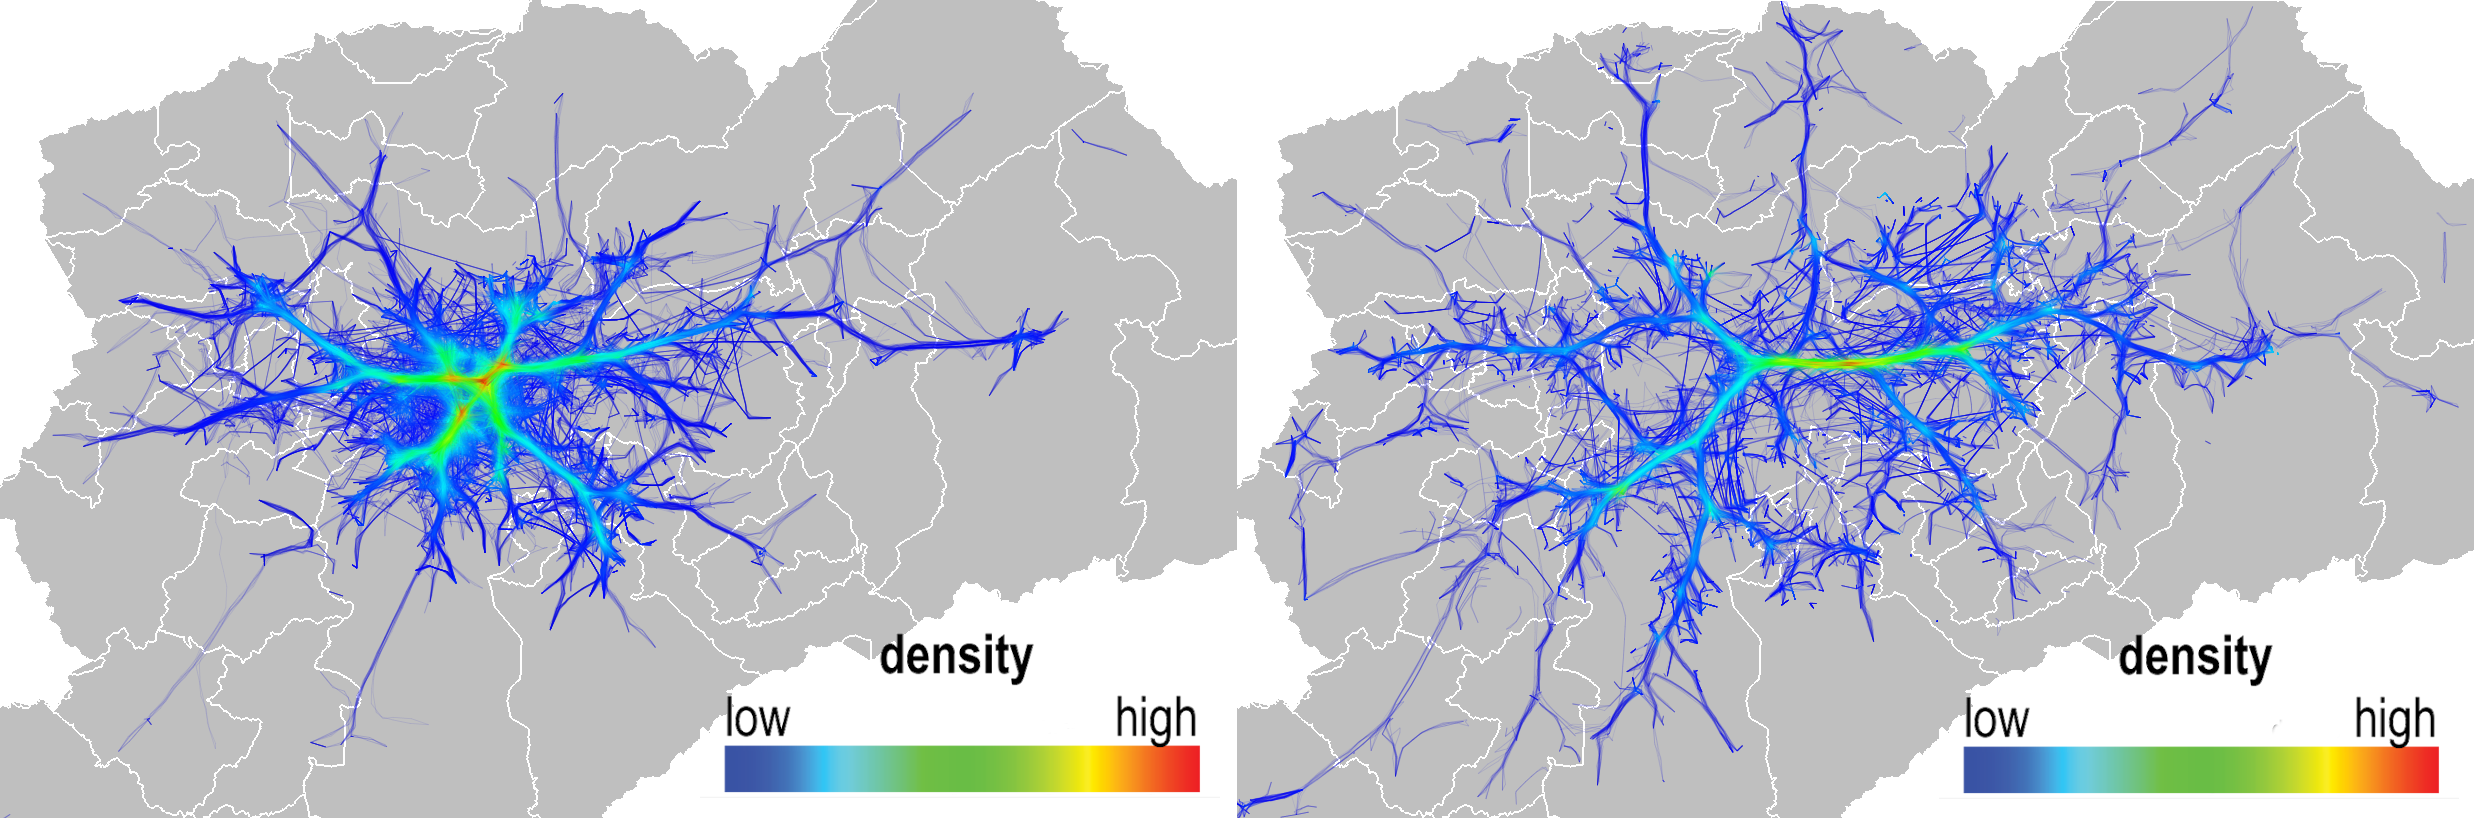
\includegraphics[width=0.98\textwidth]{../figuras/comparison-axd-e-strata-leg.png}
  \caption{Visualização da densidade. Comparação entre viagens da classe $A$ (esquerda) e $D$-$E$ (direta). \label{fig:becc-axd-e}}
\end{figure}


\begin{figure}[!htb]
  \centering
  \captionsetup{justification=centering}
  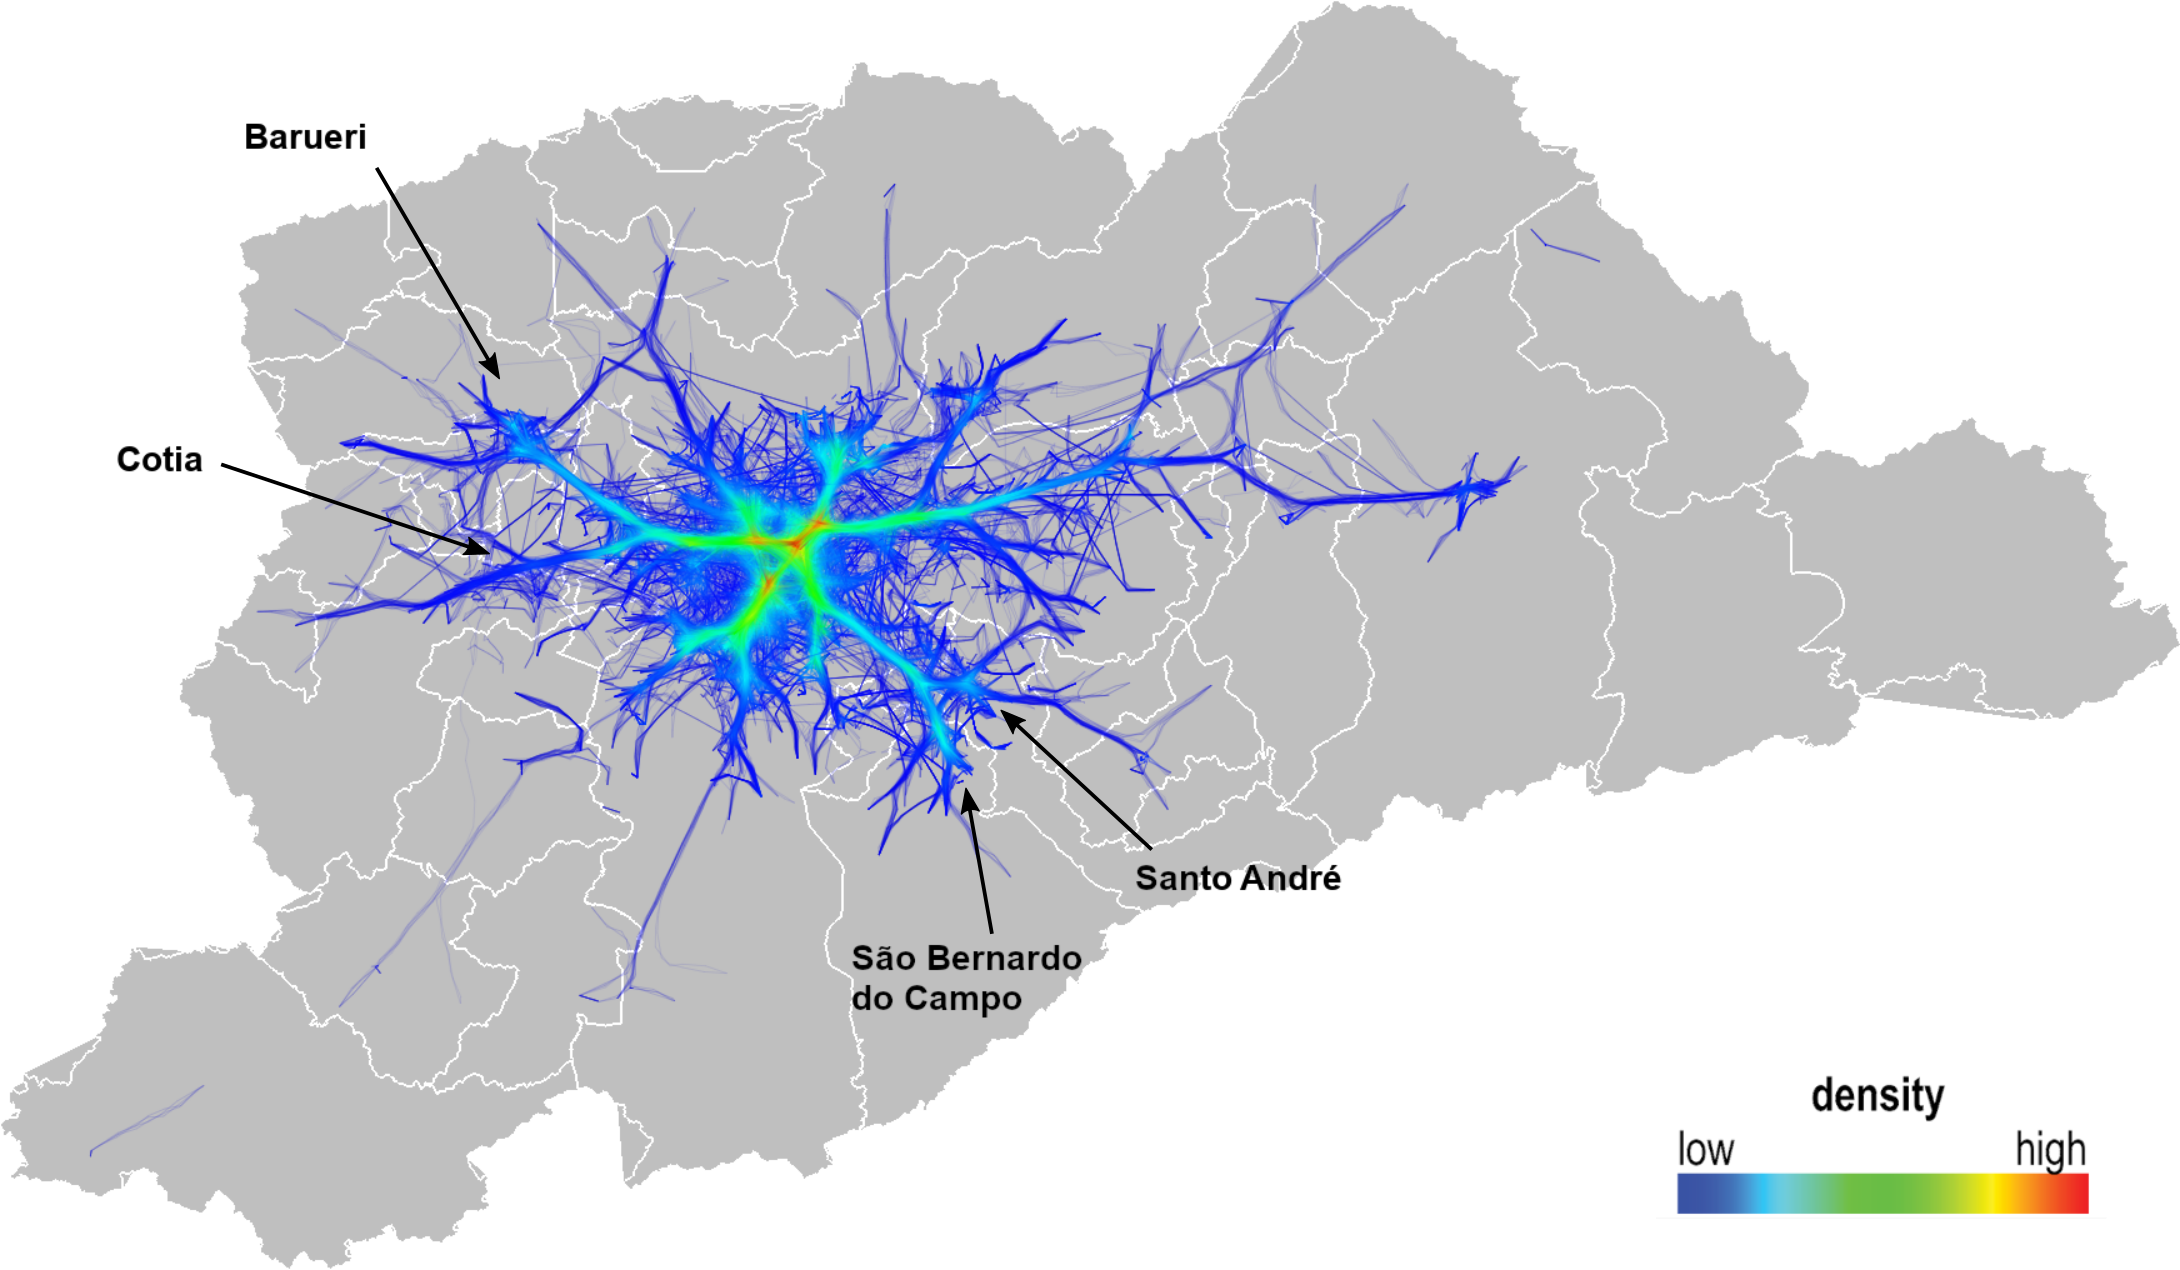
\includegraphics[width=0.98\textwidth]{../figuras/1-class-a.png}
  \caption{Densidade das viagens da classe $A$. \label{fig:becc-a}}
\end{figure}

\begin{figure}[!htb]
  \centering
  \captionsetup{justification=centering}
  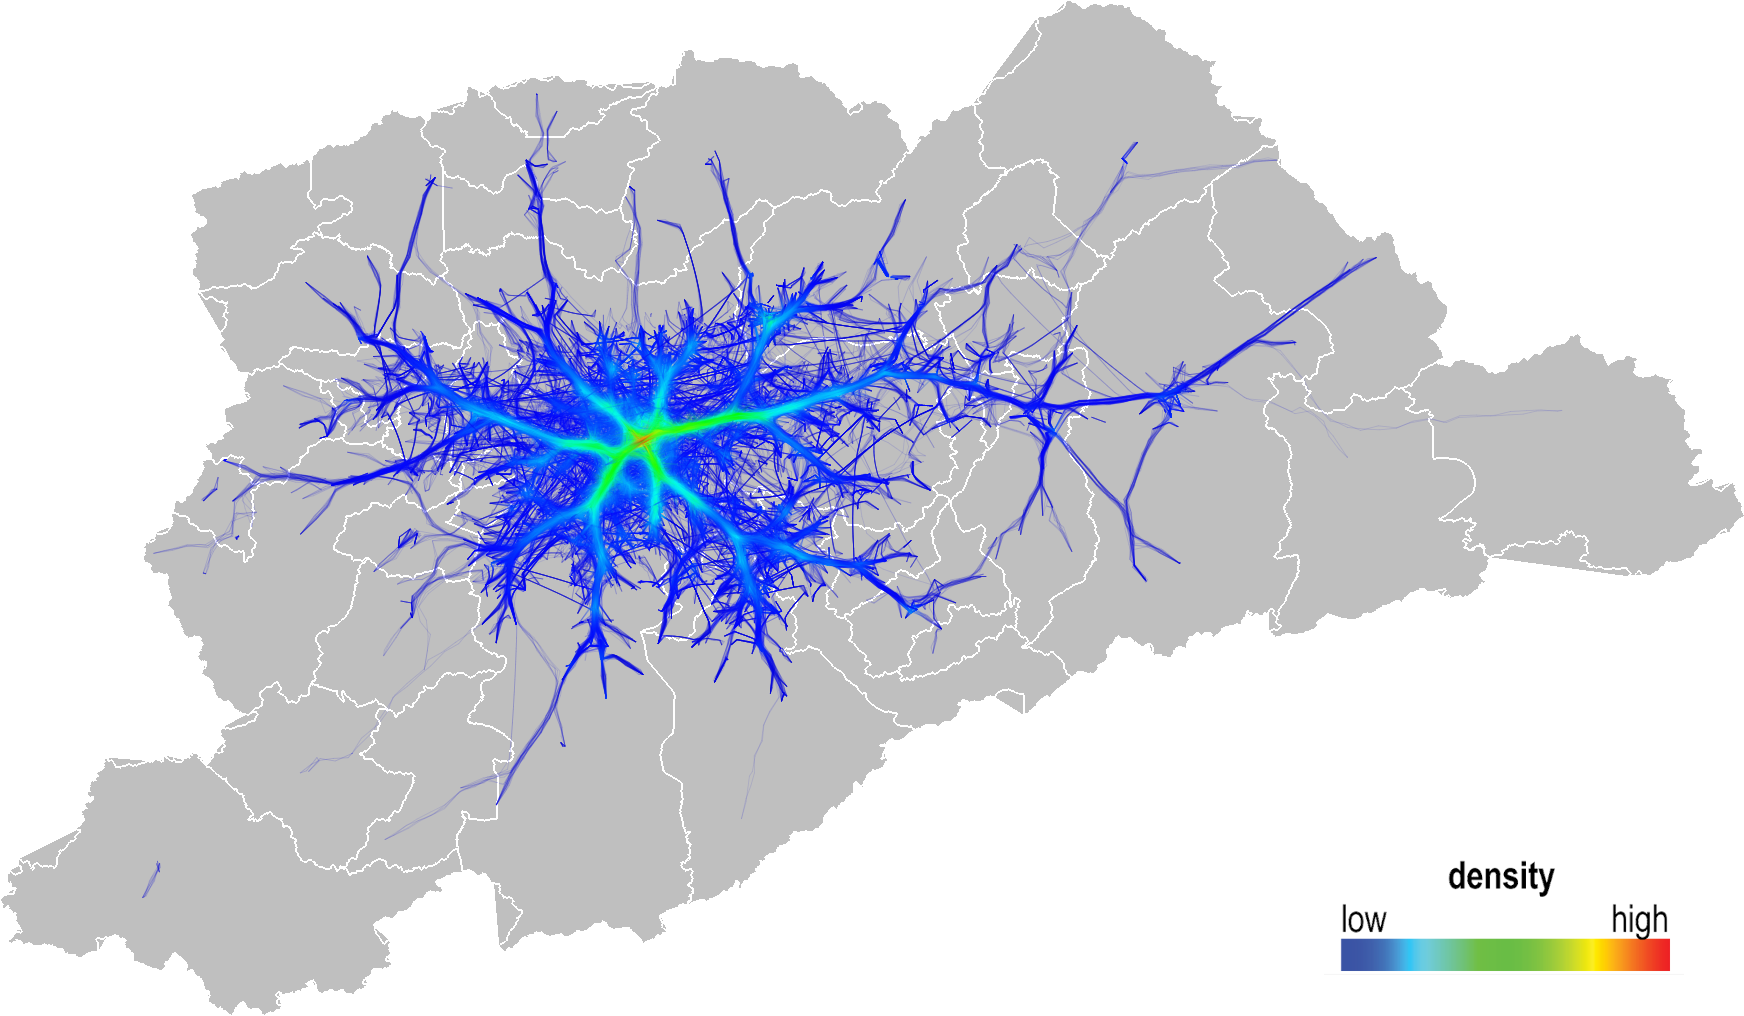
\includegraphics[width=0.98\textwidth]{../figuras/2-class-b1.png}
  \caption{Densidade das viagens da classe $B1$. \label{fig:becc-b1}}
\end{figure}

\begin{figure}[!htb]
  \centering
  \captionsetup{justification=centering}
  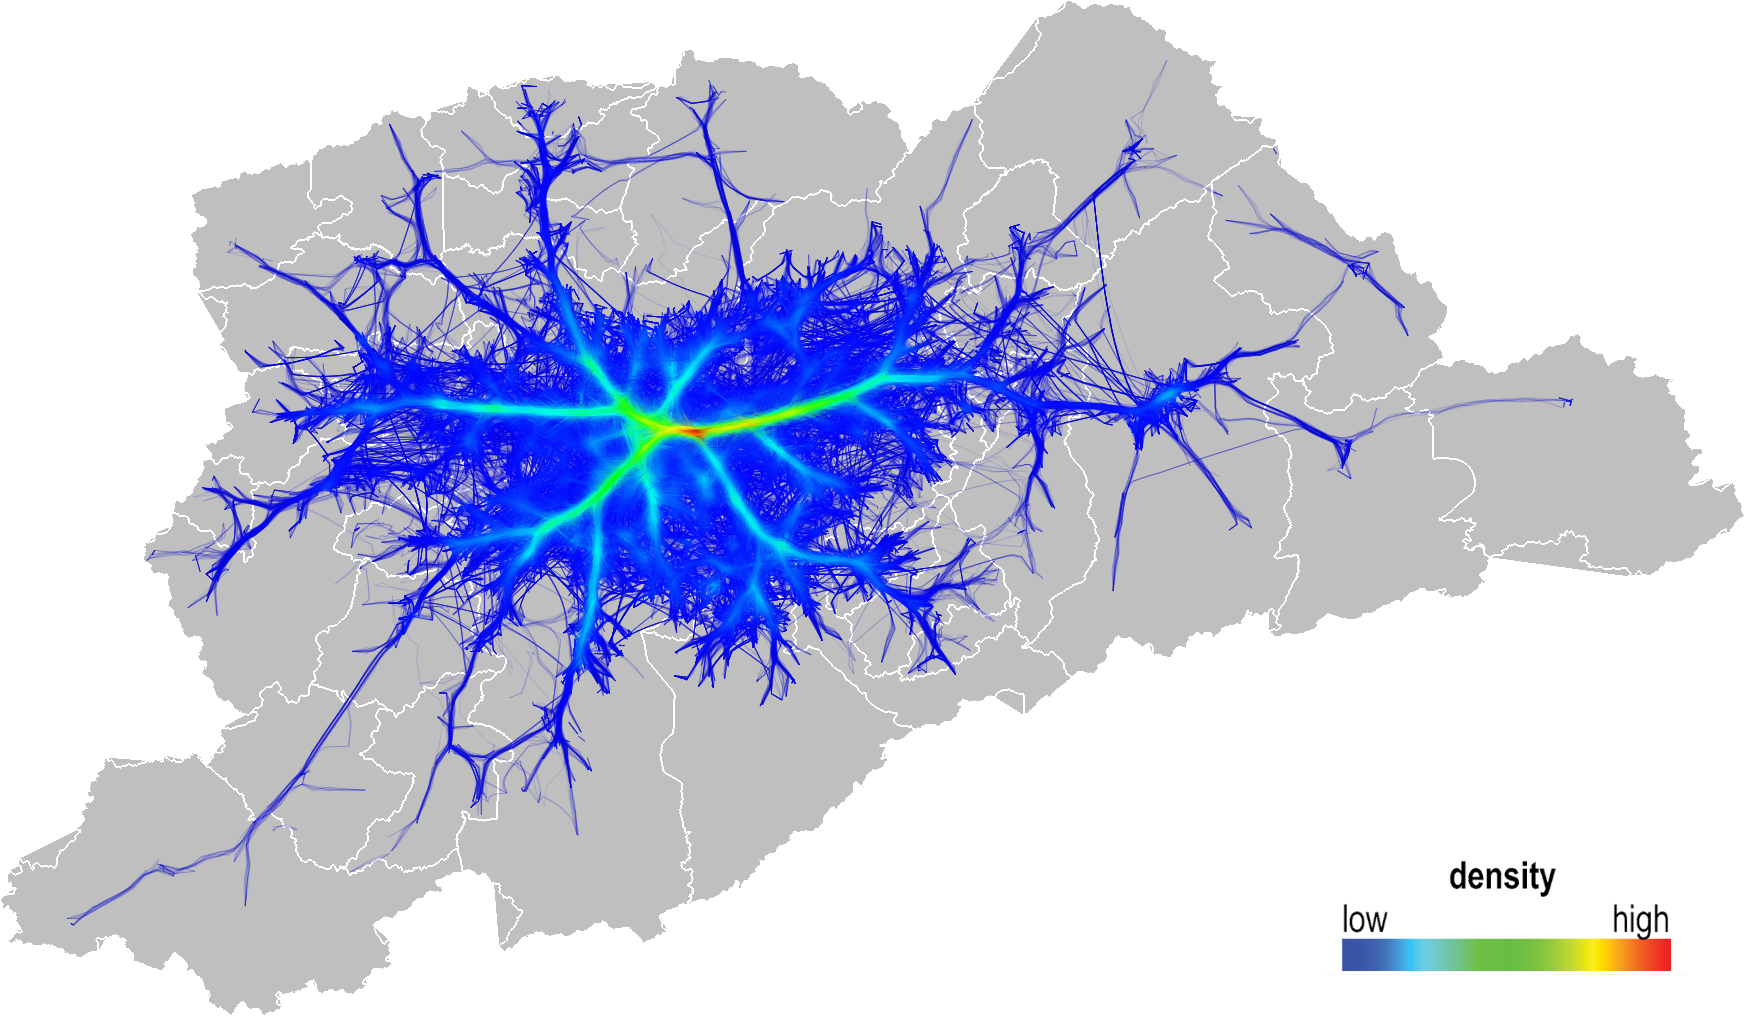
\includegraphics[width=0.98\textwidth]{../figuras/3-class-b2.png}
  \caption{Densidade das viagens da classe $B2$. \label{fig:becc-b2}}
\end{figure}

\begin{figure}[!htb]
  \centering
  \captionsetup{justification=centering}
  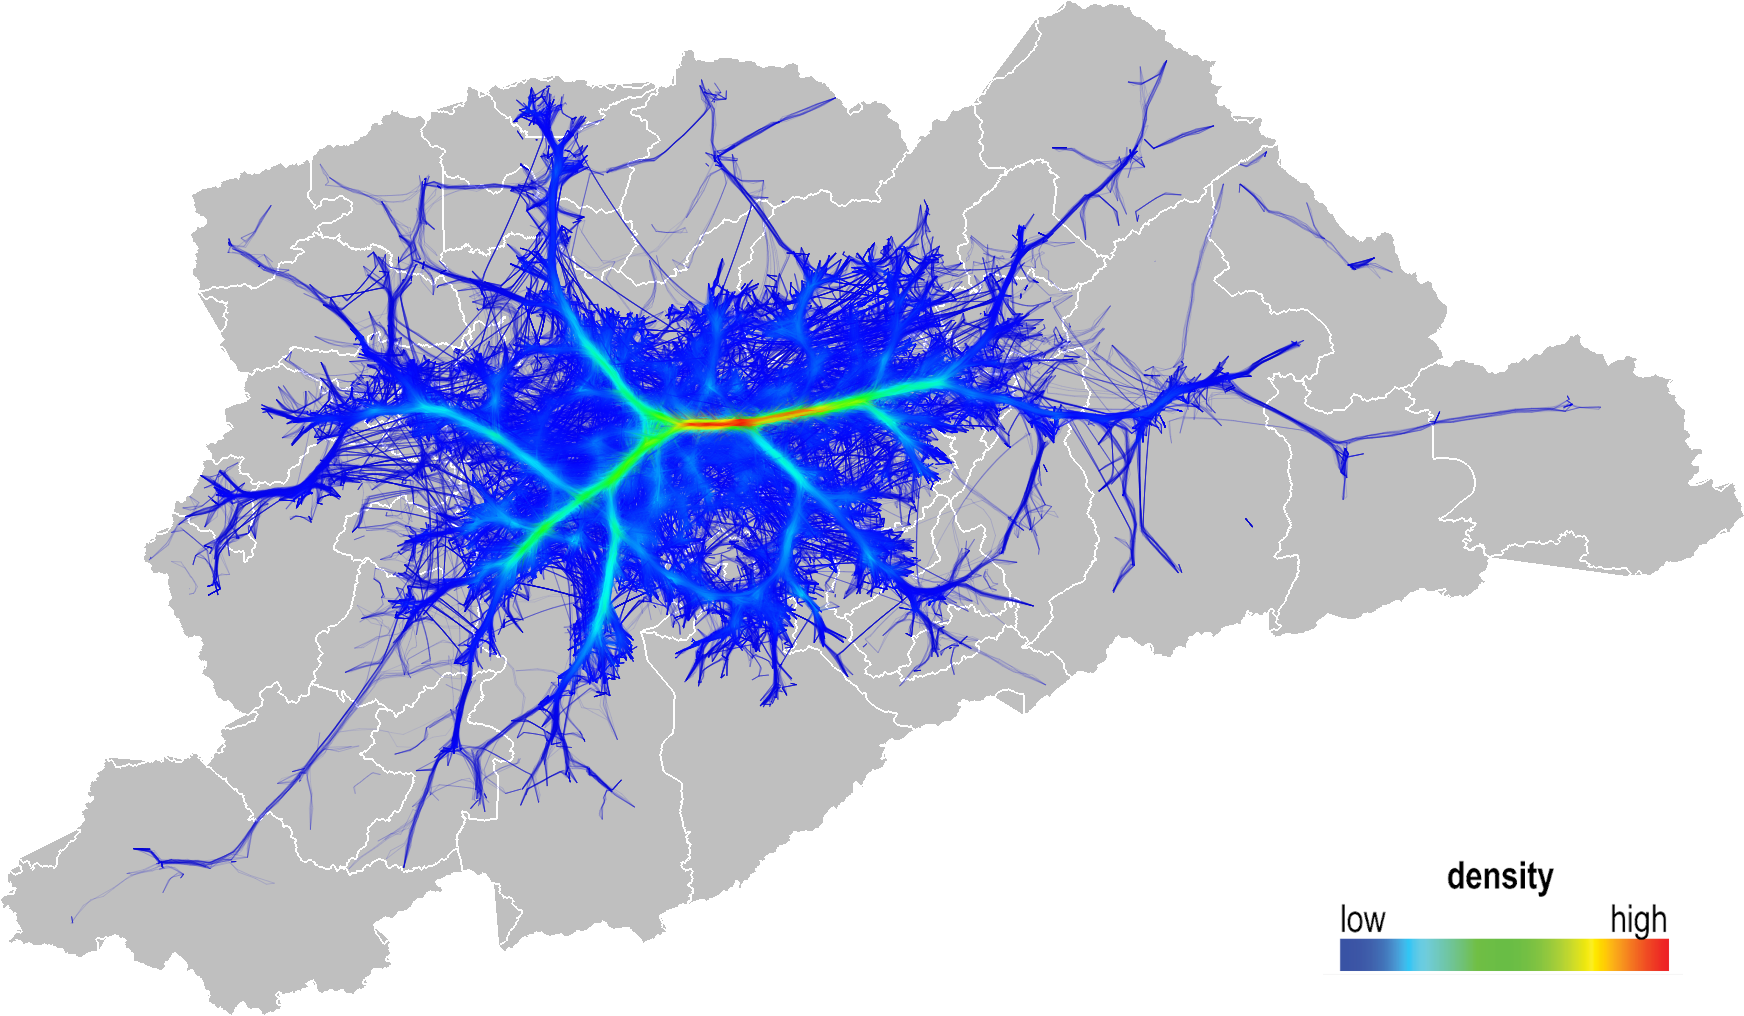
\includegraphics[width=0.98\textwidth]{../figuras/4-class-c1.png}
  \caption{Densidade das viagens da classe $C1$. \label{fig:becc-c1}}
\end{figure}

\begin{figure}[!htb]
  \centering
  \captionsetup{justification=centering}
  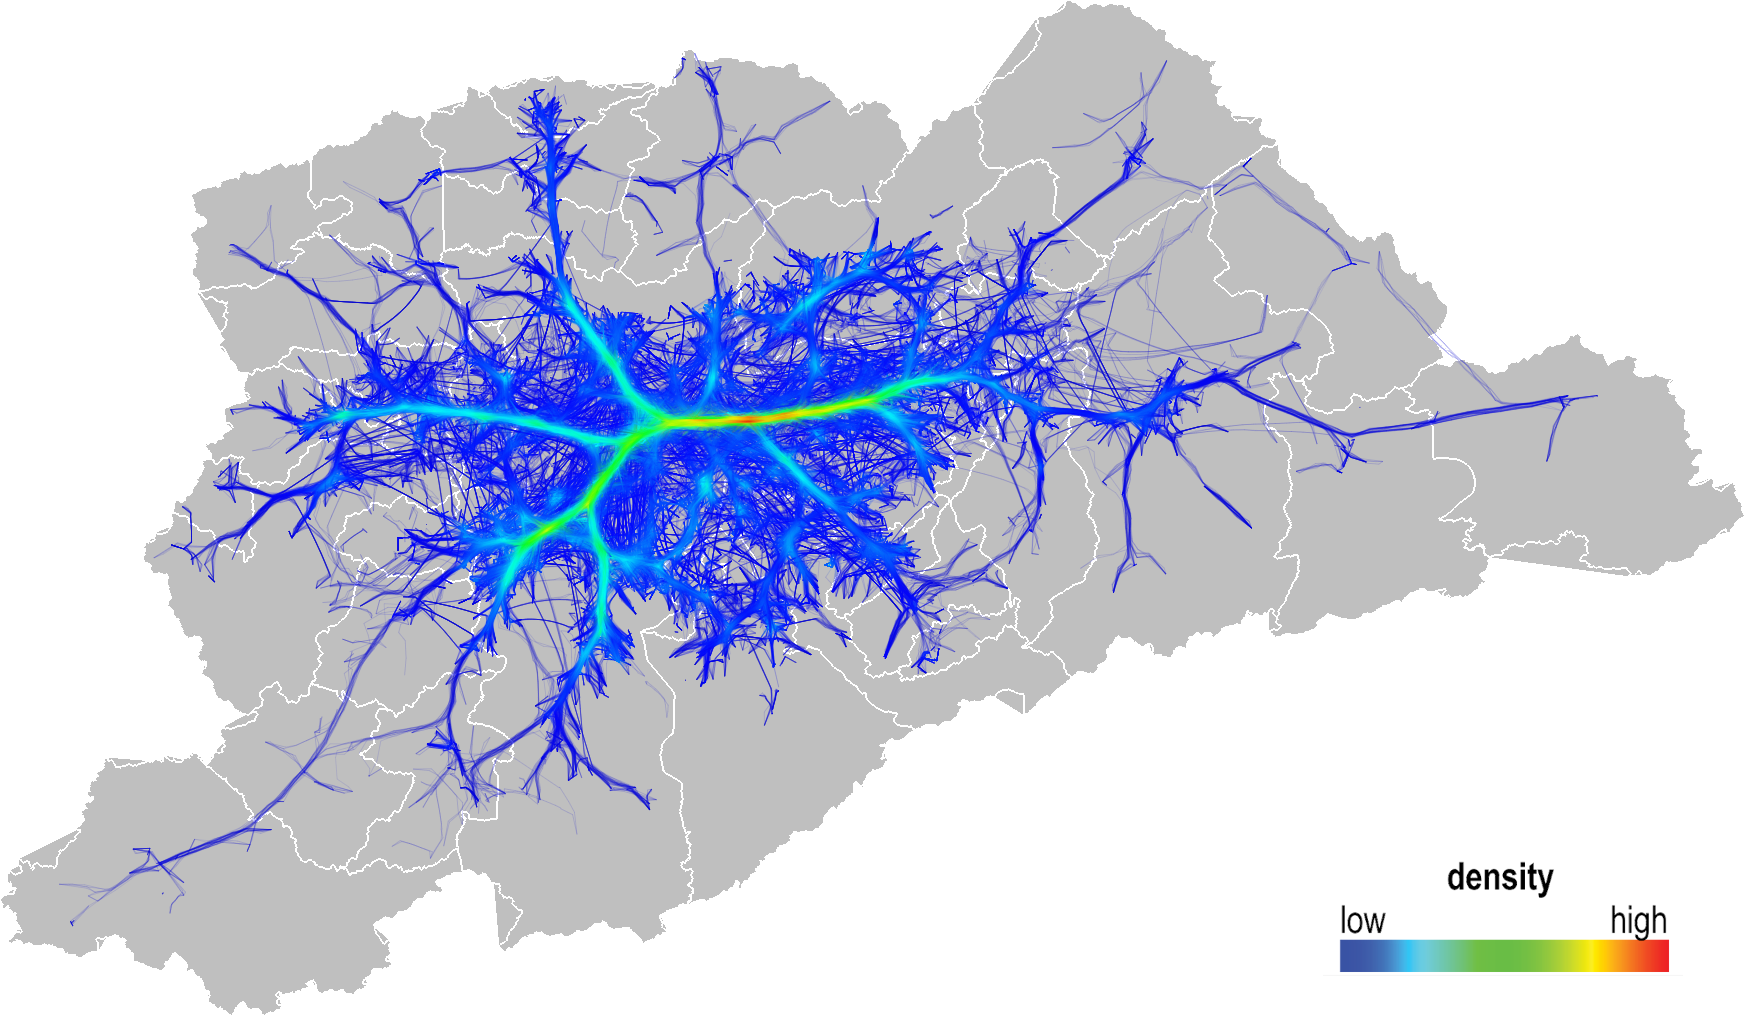
\includegraphics[width=0.98\textwidth]{../figuras/5-class-c2.png}
  \caption{Densidade das viagens da classe $C2$. \label{fig:becc-c2}}
\end{figure}

\begin{figure}[!htb]
  \centering
  \captionsetup{justification=centering}
  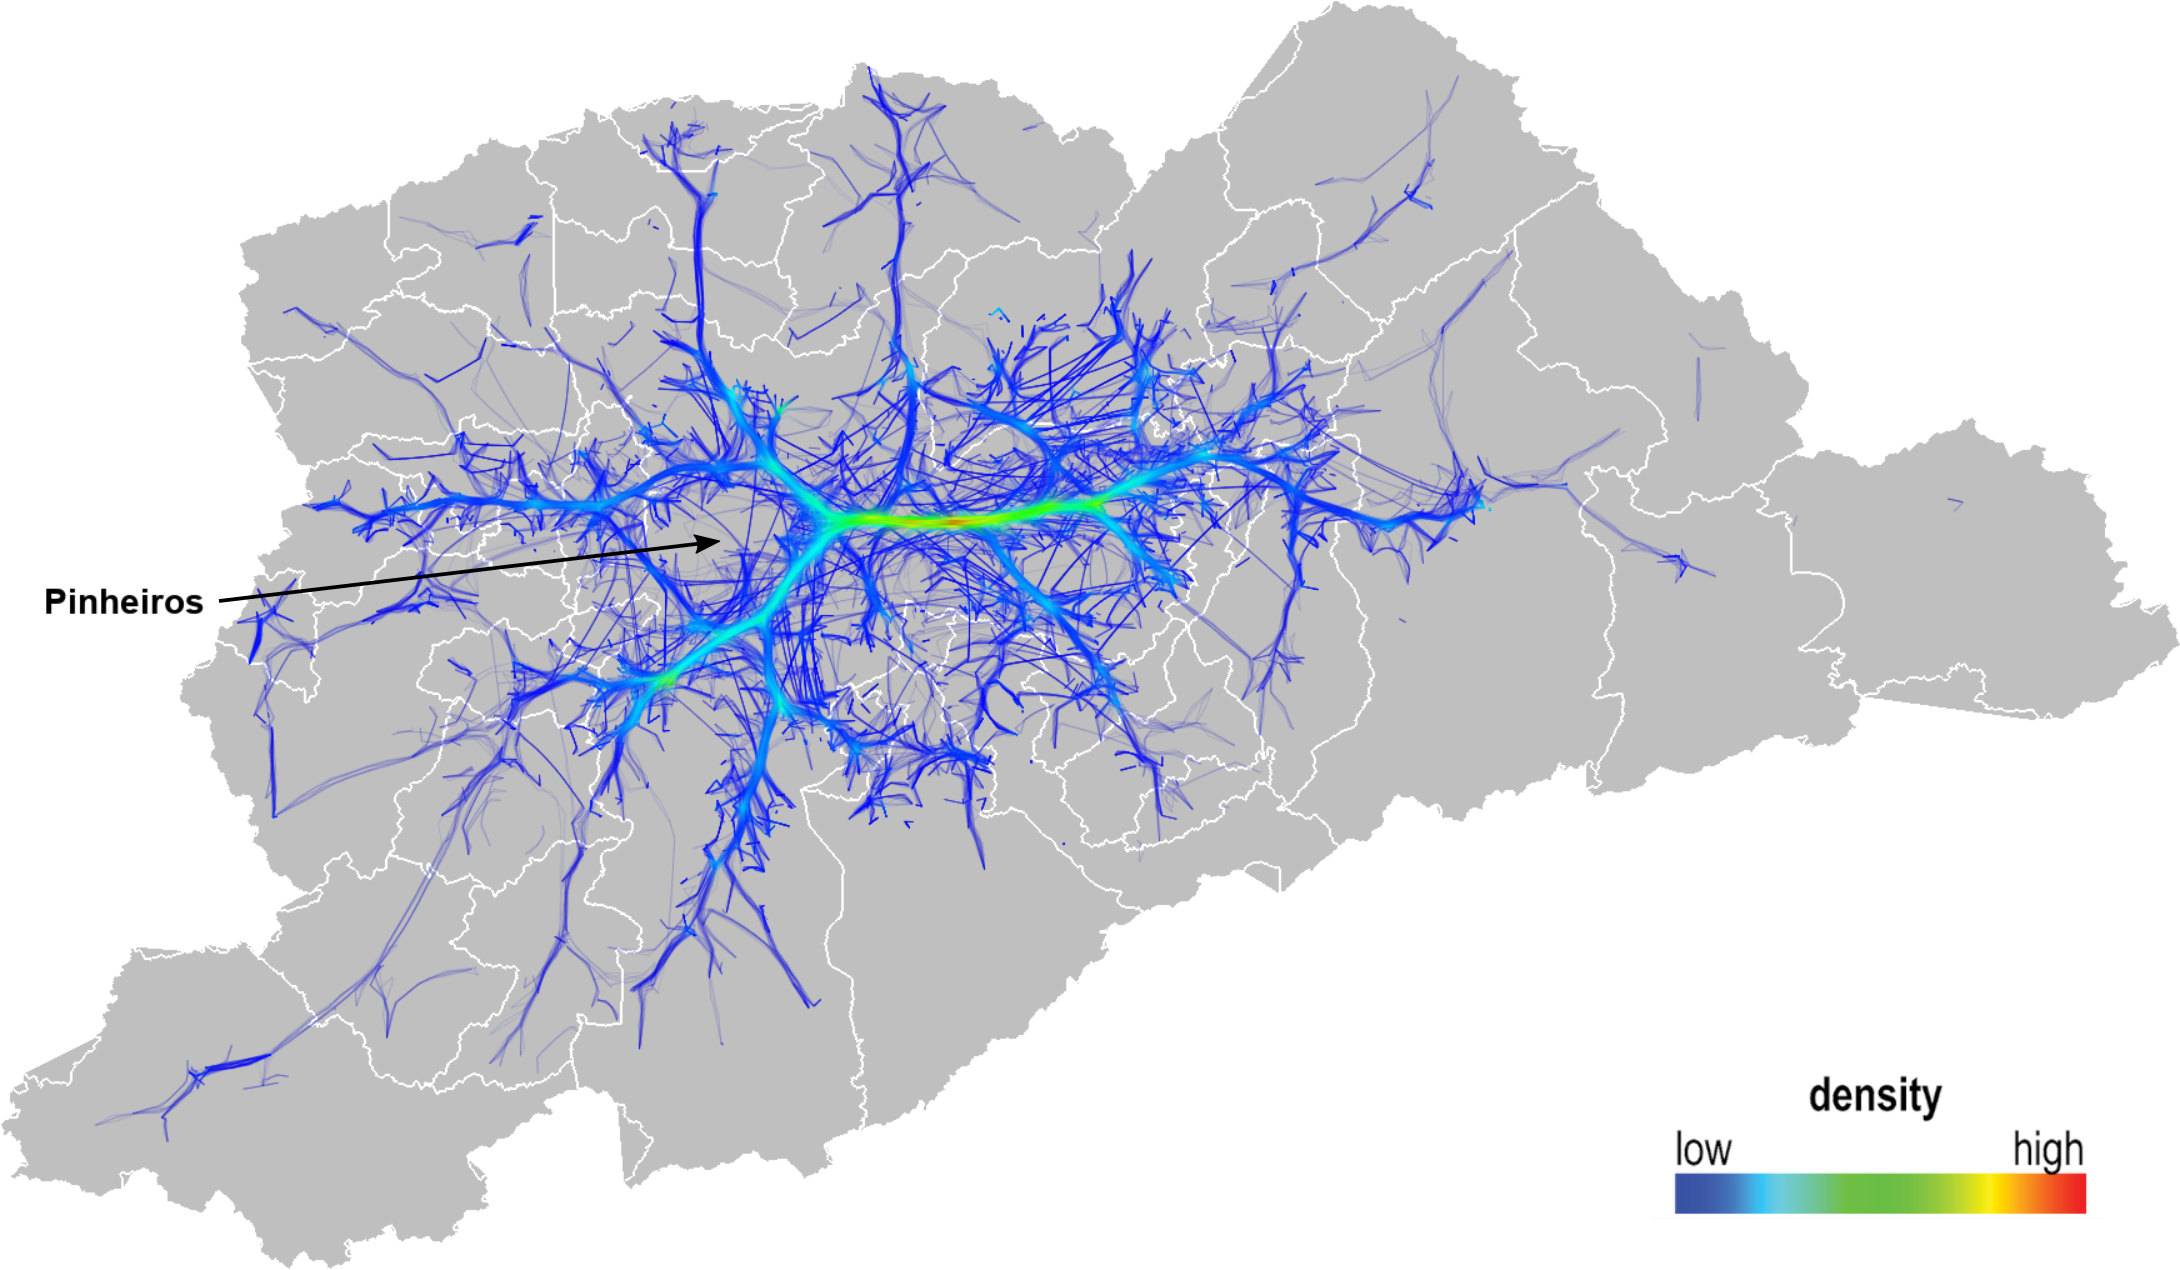
\includegraphics[width=0.98\textwidth]{../figuras/6-class-d-e.png}
  \caption{Densidade das viagens da classe $D$-$E$. \label{fig:becc-d-e}}
\end{figure}

Quando comparamos todos os mapas do nível $A$ ao $D-E$
(Figuras~\ref{fig:becc-a}~to~\ref{fig:becc-d-e}), vemos que os fluxos mais
densos (em vermelho) tendem a se deslocar do centro da capital para a região
leste da cidade. A concentração de fluxos de alta densidade está se espalhando
cada vez mais do centro para as regiões periféricas da RMSP. Mesmo os fluxos
menos densos estão aumentando e se espalhando pela RMSP. No entanto, o mapa
$D-E$ mostra que esses fluxos diminuem consideravelmente para esses estratos
sociais. Isso pode indicar que os cidadãos de baixa renda têm menos acesso ao
sistema de mobilidade urbana. Com isso, essas pessoas teriam menos acesso aos
serviços sociais, educacionais, de saúde e culturais da SPMA, uma vez que esses
recursos estão concentrados nas regiões centrais das cidades. É importante
notar que essas regiões centrais também têm mais oportunidades de emprego.
Olhando o mapa $D-E$, podemos ver um notável espaço vazio no centro oeste da capital. Essa
região (distrito de Pinheiros) concentra um grande número de empregos
relacionados à tecnologia da informação e serviços financeiros, o que requer
trabalhadores com níveis de escolaridade alto e médio. Assim, o mapa mostra que
os cidadãos de baixa renda não estão indo para aquela região, o que reflete a
desigualdade de oportunidades que esses cidadãos enfrentam.

\section{Mobility of young students from different social strata}
\label{sec:students}
% % od17-escola-alta-renda-6-18, od17-escola-baixa-renda-6-18 density1
% To explore even more the mobility patterns showed bundling visualizations, we compared the trips of students from different social strata. We filtered citizens with age between 6 and 18 years whose commuting reason is study. We split them into two groups, the high- to moderate-income, which includes the BECC levels $A$, $B1$, $B2$, and $C1$; and the low-income, which includes levels $C2$ and $D$-$E$. Figures~\ref{fig:students-high}~and~\ref{fig:students-low} show the density maps for both groups.

% \begin{figure}[!htb]
%   \centering
%   \captionsetup{justification=centering}
%   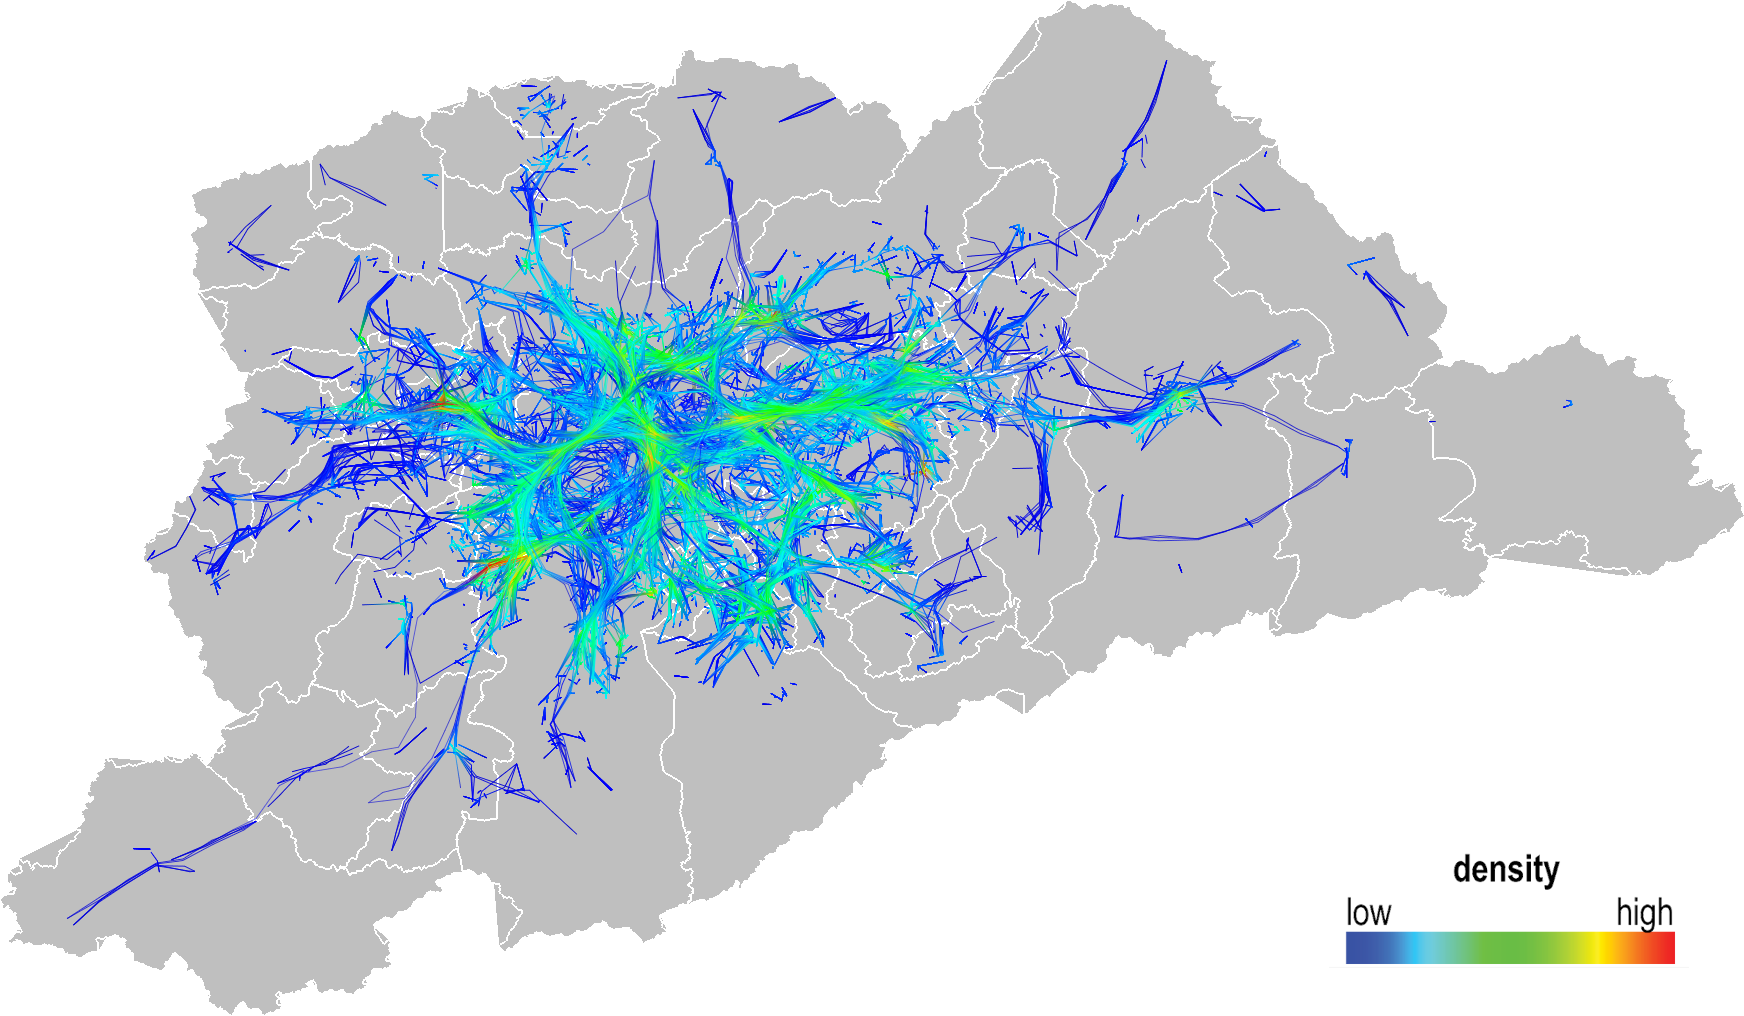
\includegraphics[width=0.98\textwidth]{figures/high-income-density-leg.png}
%   \caption{Density of trails of young students from high-income households. \label{fig:students-high}}
% %\end{figure}
% \vspace*{\floatsep}
% %\begin{figure}[!htb]
%   \centering
%   \captionsetup{justification=centering}
%   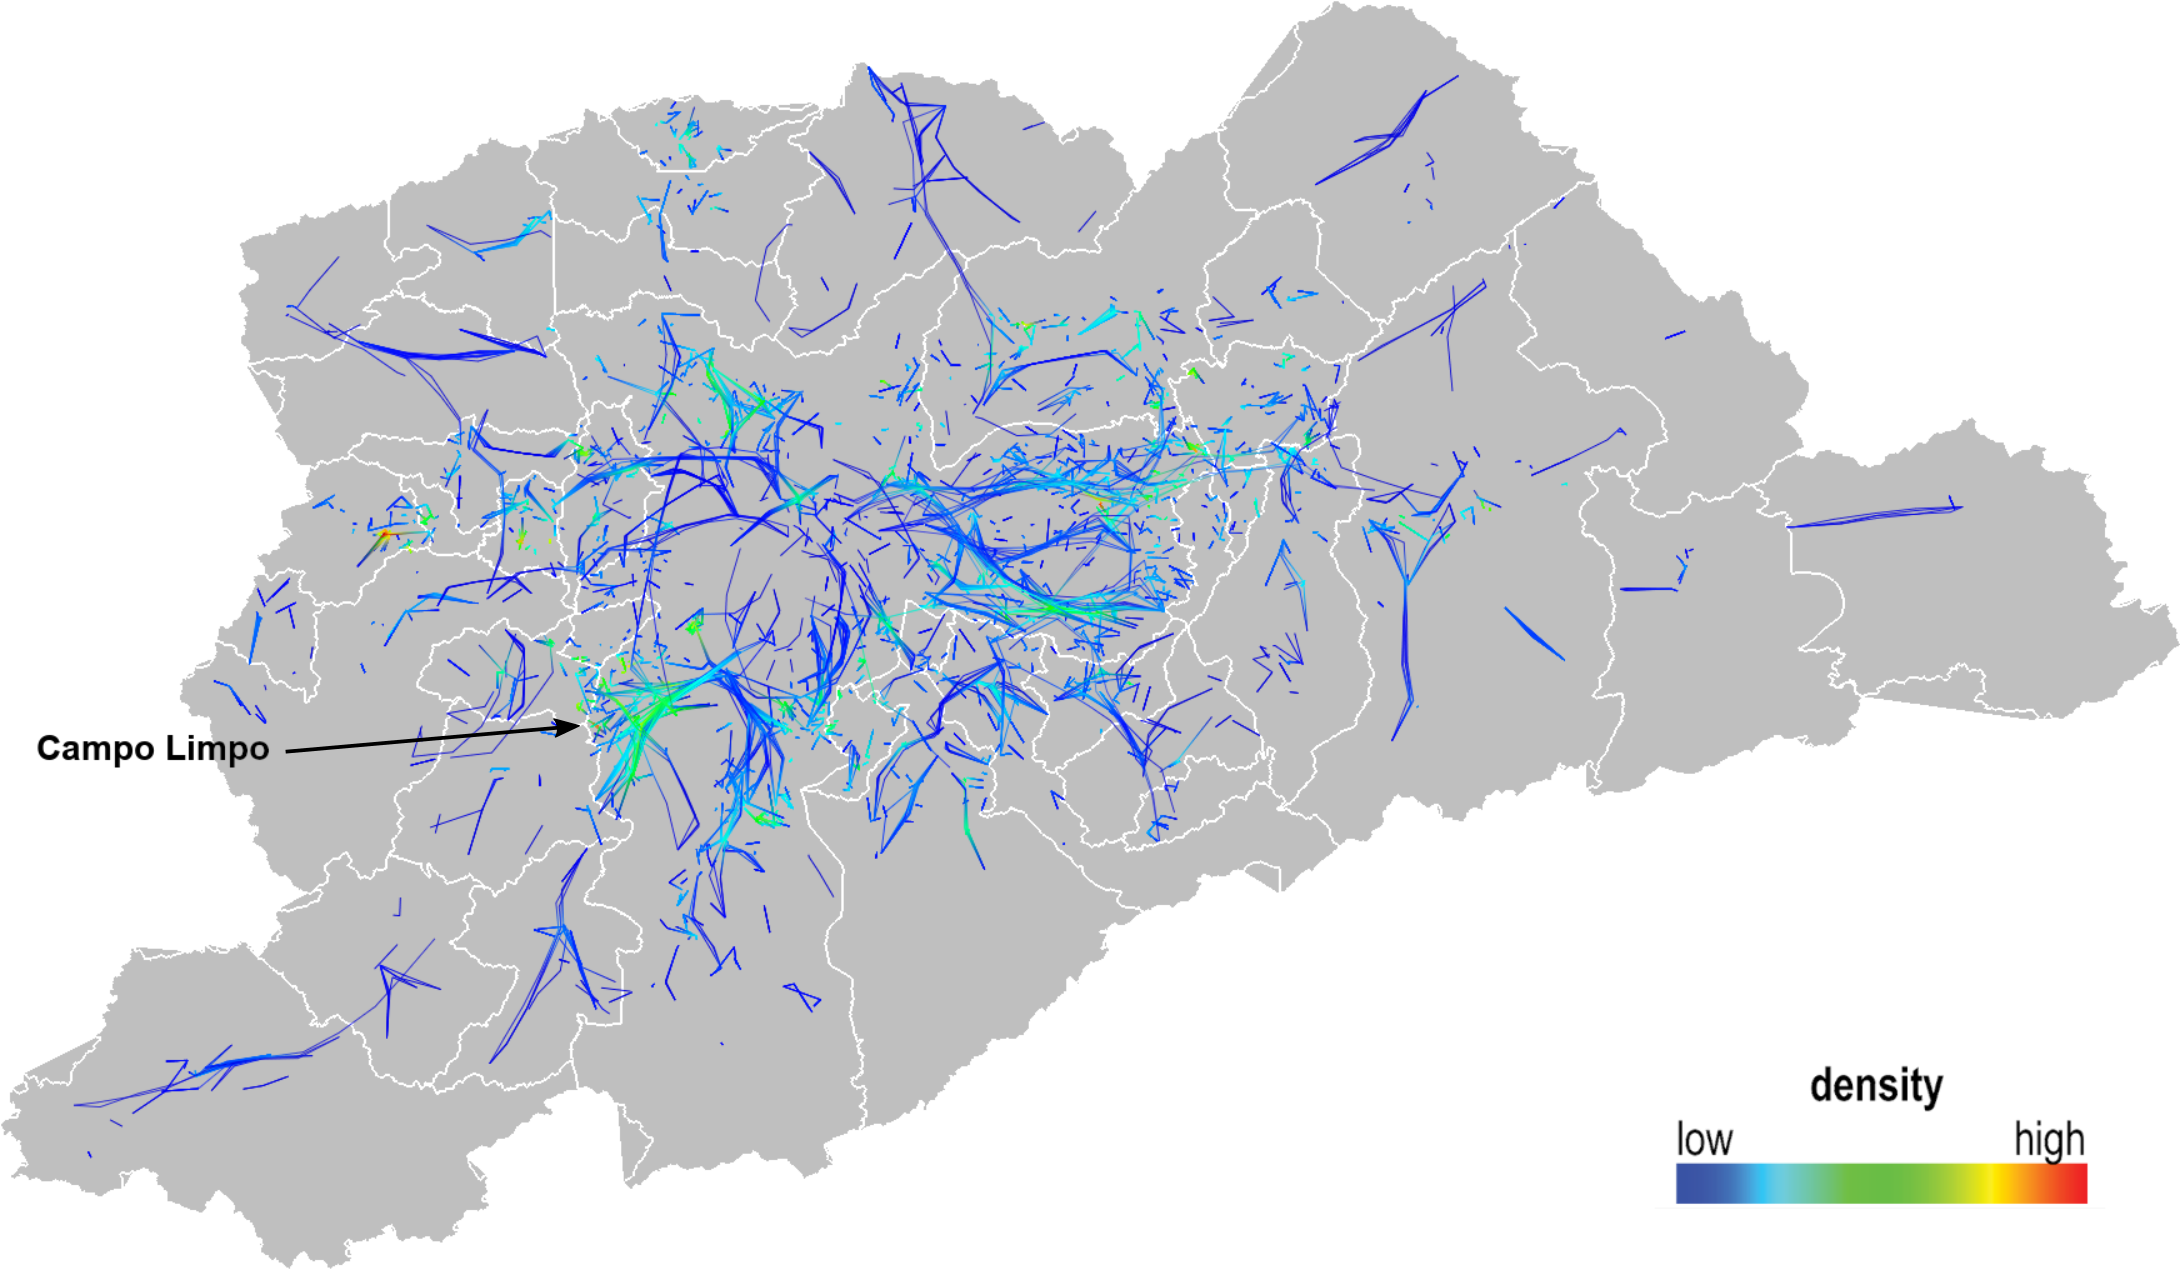
\includegraphics[width=0.98\textwidth]{figures/low-income-density-leg.png}
%   \caption{Density of trails of young students from low-income households. \label{fig:students-low}}
% \end{figure}

% The density map of the high- to moderate-income students (Figure~\ref{fig:students-high}) shows a large number of dense flows spread across the central region of SPMA. This part of SPMA concentrates most private schools, universities, and complementary colleges. In addition, high density flows are not as long as flows from other maps with all the data (e.g., Figure~\ref{fig:bundled-graph-density}). This indicates that trips to study are shorter than trips to work. 

% The density map of low-income students (Figure~\ref{fig:students-low}) shows that their mobility is very limited compared to the higher-income students. There are a few dense flows, most of them out of the capital downtown. The high density flows of low-income students are more present in the peripherals of the capital and also in the neighboring cities. There is a concentration of both groups in the southwest region, where are the neighborhoods of the Campo Limpo district. 

% It is worthy to note that the public schools in the SPMA are spread across the central and peripheral parts of the cities. The students are enrolled in these schools according to the proximity of their residences. Thus, they do not have to travel long distances to reach their schools. Also, public schools have lower educational performance than private schools in S\~ao Paulo. Thus, citizens with better financial conditions use to put their children in private schools.

% The scarcity of flows from low-income students may indicate that they do not have equal opportunities to study, being enrolled in schools in their neighborhood. They also do not use to go to the central region of the city and, thus, have less access to universities and complementary colleges. This inequality of opportunities will probably impact these students' jobs and economical conditions.

% We also see that there are many more trails for the high- to moderate-income students (Figure~\ref{fig:students-high}) than for low-income students (Figure~\ref{fig:students-low}). The high-to moderate-income students also travel large distances to study, which indicates that they can choose more flexibly where to study. This fact is corroborated by urban mobility studies that indicate that people with better financial conditions have more mobility than those with poorest conditions\,\cite{carruthers2005,lucas2016}.

\section{Directions at peak hours}
\label{sec:peak-hours}
% %
% As discussed earlier in Sec.~\ref{sec:data}, Figure~\ref{fig:trips_by_hour} shows the distribution of trips by hour of the day, with two main rush-hour peaks (6-9 AM and 5-8 PM). 
% However, this aggregated table does not give us insights in how the rush-hour patterns may differ. To see this, we selected the two rush-hour time intervals and visualized them separately, using directional bundling and color-coding.

% \begin{figure}[!htb]
%   \centering
%   \captionsetup{justification=centering}
%   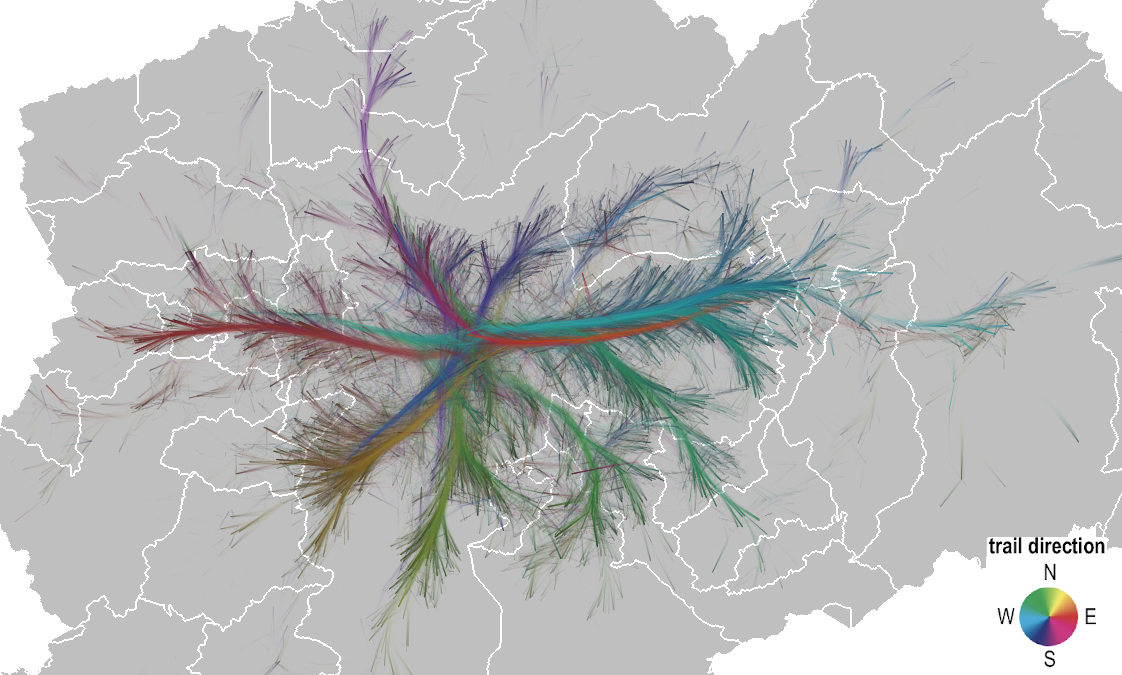
\includegraphics[width=0.98\textwidth]{figures/peak-hours-6h-to-9h-direction-leg.png}
%   \caption{Directions of trips between 6 to 9 AM \label{fig:peak-hours-6h-9h}}
% %\end{figure}
% \vspace*{\floatsep}
% %\begin{figure}[!htb]
%   \centering
%   \captionsetup{justification=centering}
%   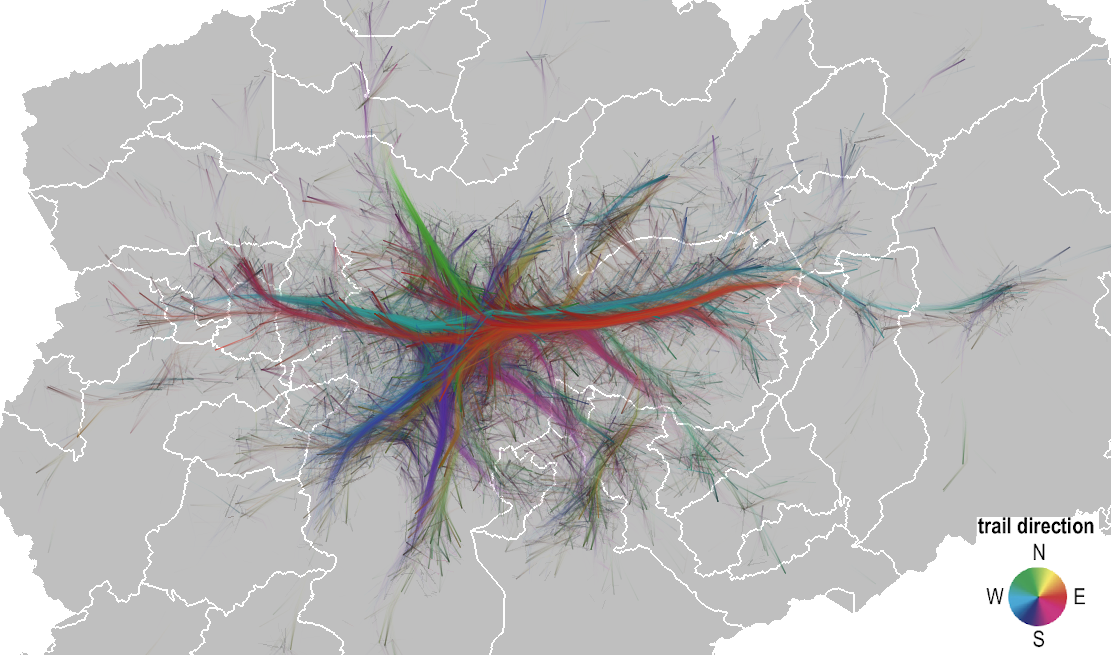
\includegraphics[width=0.98\textwidth]{figures/peak-hours-17h-to-20h-direction-leg.png}
%   \caption{Directions of trips between 5 to 8 PM \label{fig:peak-hours-17h-20h}}
% \end{figure}

% Comparing the peak hours, we can see that morning flows going to the SPMA center (Figure~\ref{fig:peak-hours-6h-9h}, cyan bundle)
% are overall denser and longer than the flows coming from the SPMA center during the afternoon/evening peak (Figure~\ref{fig:peak-hours-17h-20h}, red). This suggests that in the morning people are in a hurry to reach their work, while they are less in a hurry to go back home (or to other destinations like schools or the gym) in the afternoon/evening.

% In Figure~\ref{fig:peak-hours-6h-9h}, we can see that flows in the morning peak going to the capital downtown (cyan bundle coming from the east) are denser than opposite flows (red bundle going to the east). Although flows leaving the capital downtown in the morning are thinner than their opposite ones, they also concentrate a large number of trips, especially to the east and southwest. In Figure~\ref{fig:peak-hours-17h-20h}, the opposite flows seem more equally distributed.

\section{Density by transportation mode}
\label{sec:mode}
% %% on foot, bike, car, metro (sliced, density)
% We next split the OD17 data by transportation mode to compare the flow patterns for four different transportation modes: pedestrians, bicycles, cars, and subway. Figures~\ref{fig:mode-pedestrian}~to~\ref{fig:mode-subway} show the respective visualizations.

% \begin{figure}[!htb]
%   \centering
%   \captionsetup{justification=centering}
%   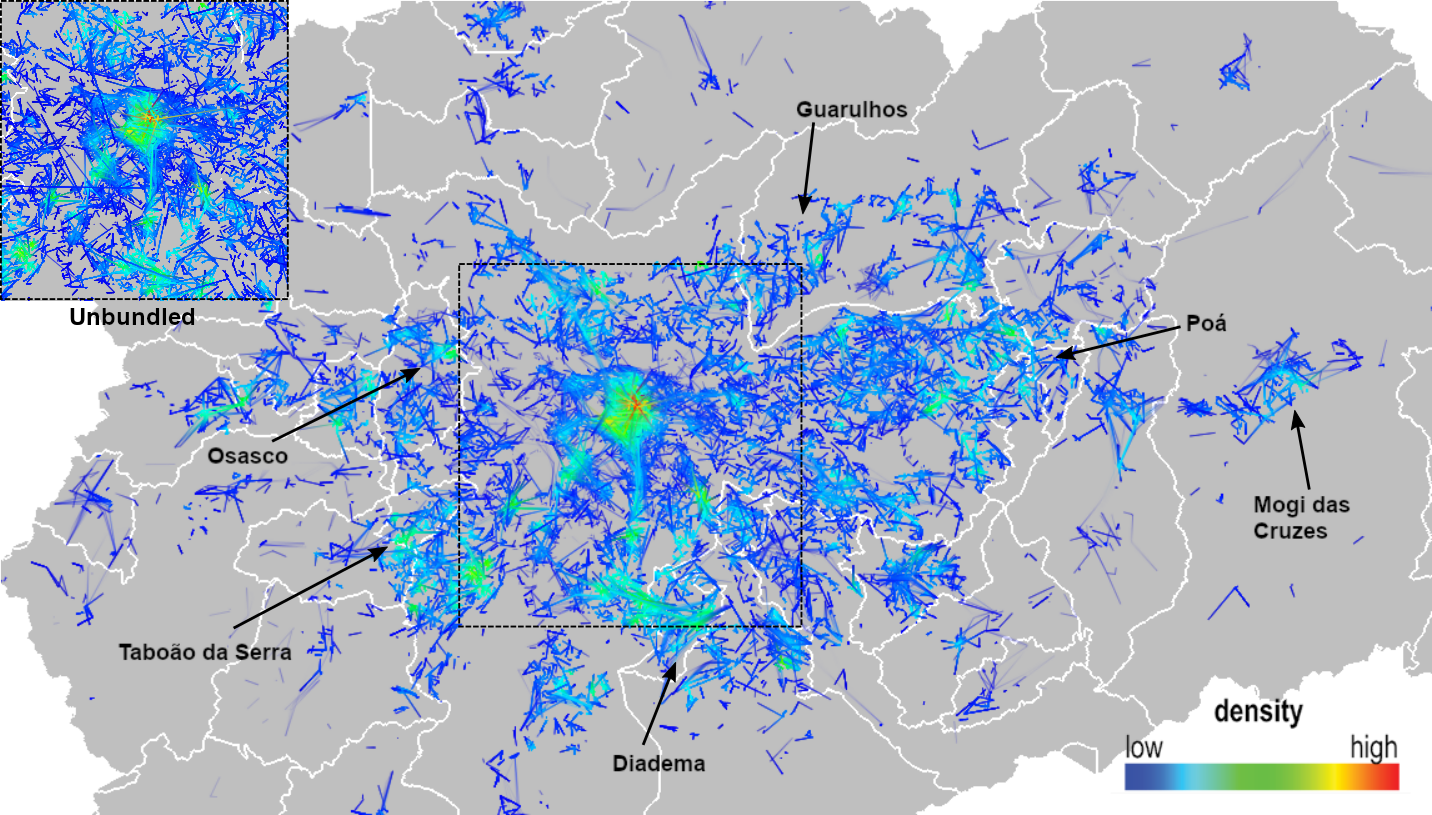
\includegraphics[width=0.98\textwidth]{figures/mode-pedestrian-density-leg.png}
%   \caption{Density of pedestrian trips \label{fig:mode-pedestrian}}
% \end{figure}

% \begin{figure}[!htb]
%   \centering
%   \captionsetup{justification=centering}
%   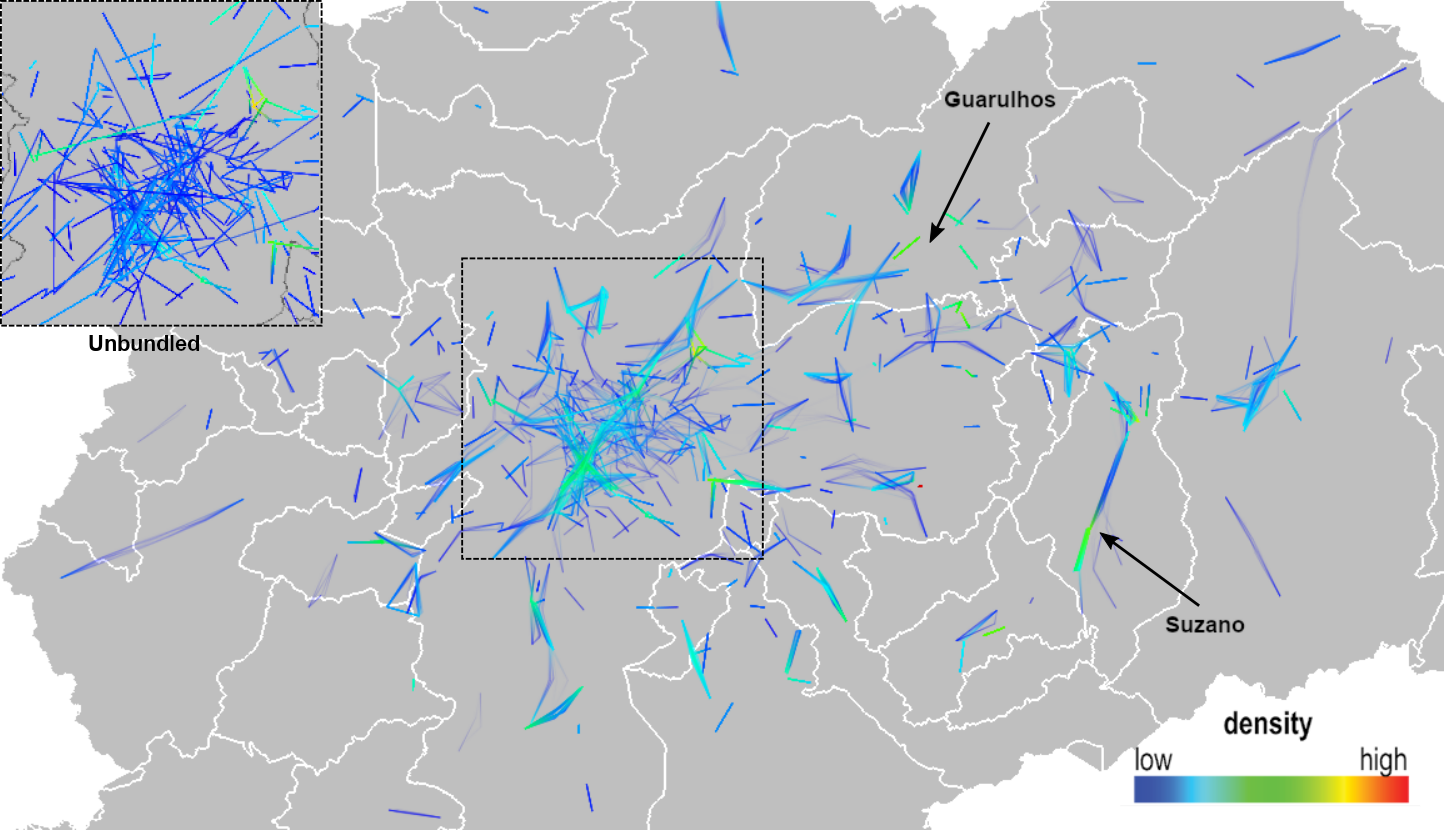
\includegraphics[width=0.98\textwidth]{figures/mode-bike-density-leg.png}
%   \caption{Density of bicycle trips \label{fig:mode-bike}}
% \end{figure}

% \begin{figure}[!htb]
%   \centering
%   \captionsetup{justification=centering}
%   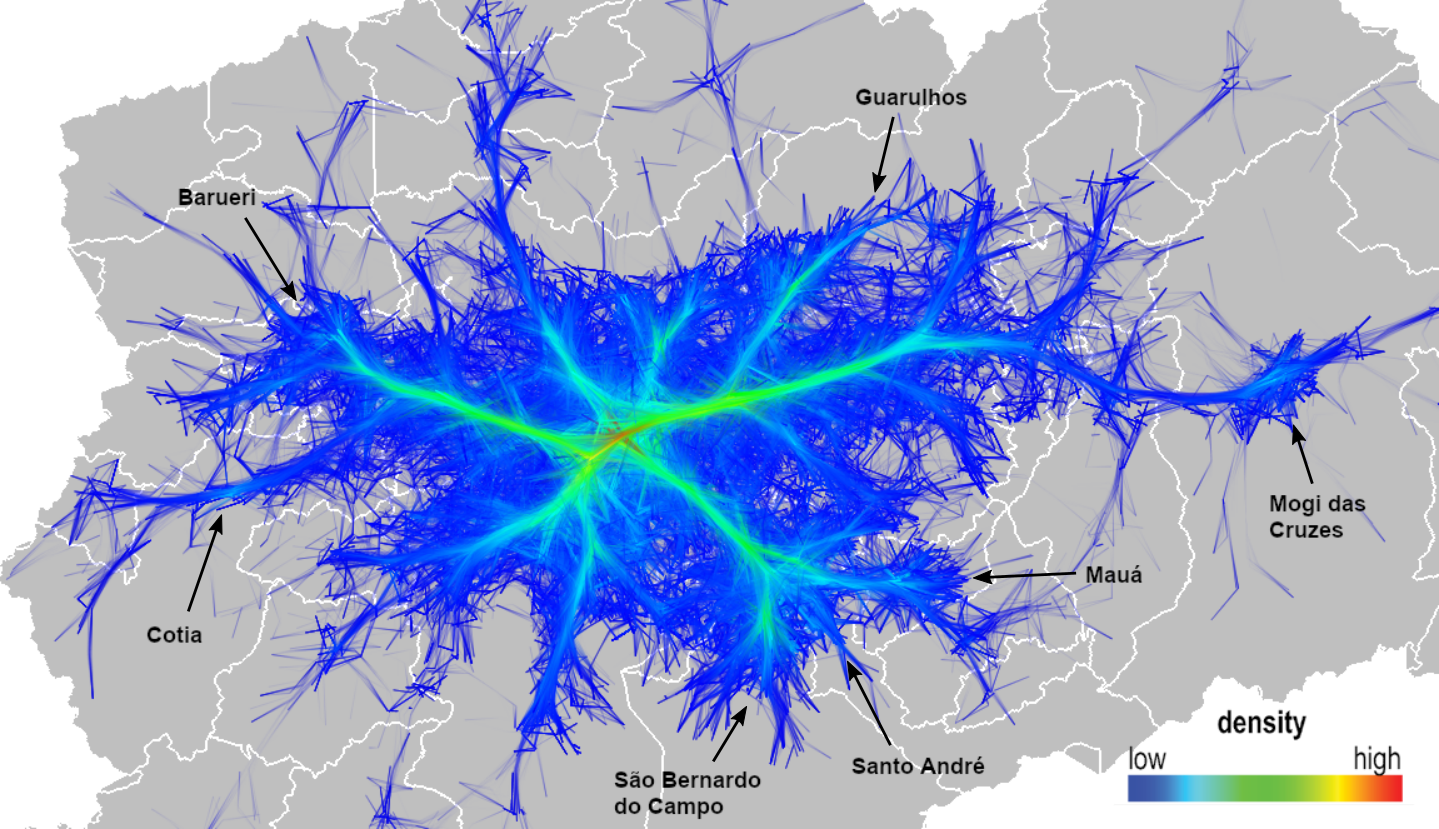
\includegraphics[width=0.98\textwidth]{figures/mode-car-density-leg.png}
%   \caption{Density of car trips \label{fig:mode-car}}
% \end{figure}

% \begin{figure}[!htb]
%   \centering
%   \captionsetup{justification=centering}
%   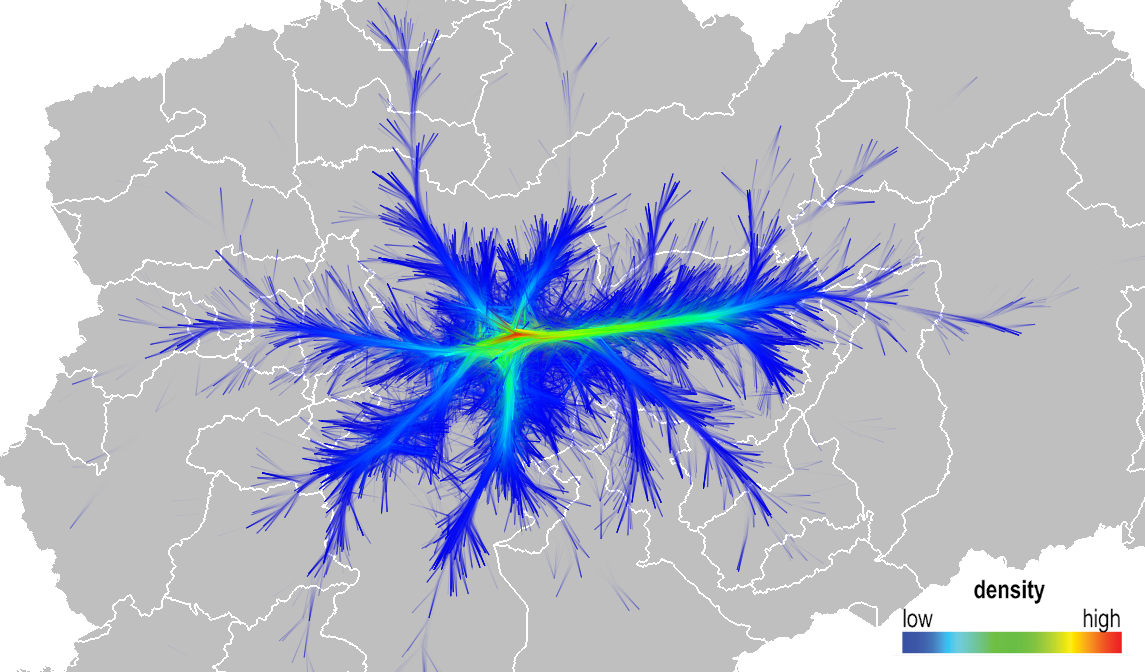
\includegraphics[width=0.98\textwidth]{figures/mode-subway-density-leg.png}
%   \caption{Density of subway trips \label{fig:mode-subway}}
% \end{figure}

% Pedestrian trails (Figure~\ref{fig:mode-pedestrian}) form several low-density `islands' spread across the SPMA, with the densest one (red in figure) being in the capital downtown. Most trails are quite short, which is expected (pedestrians). However, we see a few longer bundles between the capital downtown and the south and north regions of the city. Dense flows are also present in the neighboring cities of Diadema, Tabo\~ao da Serra, Osasco, Guarulhos, Po\'a, and Mogi das Cruzes. Upon examination, we found these dense flows to match the cities' downtown and commercial areas. This information could be useful to find places that could deserve the attention of local governments to provide improvements for pedestrians.

% As most of the pedestrian trips are short, the bundling technique forms a few flows over the SPMA.
% Using bundling for those short trips result in low-density trails, which is less useful compared to long trips. Thus, in these cases it may not be necessary to use bundling. In the upper left area of Figure~\ref{fig:mode-pedestrian}, we can see the OD trails without using bundling, which are near identical to the main bundled area.
% %For pedestrian trails, it would be interesting to apply bundling over small areas. \textbf{AT: Actually, you can do this by running CUBu simply using a much smaller kernel size. But, if we do not do that, I think we should omit the above sentence.}

% Bicycle trips (Figure~\ref{fig:mode-bike}) exhibit similar patterns to pedestrian ones. They are shorter than three kilometers on average. In this figure, we see some thin flows in the capital downtown area. There are also some more salient flows in the capital northeast and in the neighboring cities of Suzano and Guarulhos.
% However, comparing Figure~\ref{fig:mode-bike} with all other transportation means, we immediately see that bicycle trips are by far the least numerous, and exhibit a far sparser pattern, with few star-shaped `hubs' where many trails meet. This suggests that the cycling infrastructure is quite limited, and fragmented. Figure~\ref{fig:mode-bike} also shows trails without using bundling in the upper left corner.

% The car trips (Figure~\ref{fig:mode-car}) show a pattern similar to the one displaying the entire dataset, \emph{i.e.}, all transportation modes (see \emph{e.g.} Figure~\ref{fig:bundled-graph-density}). For a start, this tells that cars are \emph{the} dominant form of transportation in the SPMA, accounting for the main traffic patterns. The highest-density flows occur in the capital downtown. There are several high-density flows linking the downtown area to the other regions of the capital, and also coming and going from the cities of Guarulhos, Barueri, Cotia, S\~ao Bernardo do Campo, Santo Andr\'e, Mau\'a, and Mogi das Cruzes. Compared to all other transportation modes, cars show a far more `spread out' pattern that covers very large areas, indicating that cars are the prevalent transportation mode in most parts of the SPMA.

% Finally, subway trips (Figure~\ref{fig:mode-subway}) show a strong star-shaped pattern, with very high density bundles that connect the capital with the neighboring cities, due to the integration of the subway system with the train system. Compared to all other transportation modes, subways show a clearer, simpler, trip pattern structure.

\section{Different trip reasons}
\label{sec:dist_reasons}
% We next aim to study whether trips done for different reasons exhibit distinct trip patterns. For this, we create bundled visualizations from the OD17 data with trips grouped by work, health, education, and shopping. Figures~\ref{fig:reason-work}~to~\ref{fig:reason-shopping} show the results.

% Work-related trips (Figure~\ref{fig:reason-work}) are overall longer than the other trip reasons, and also cover a larger area (see the central agglomeration in the figure). Interestingly, the longest trips, between the east side and the city center (red bundle), are similar in pattern to the longest trips for health and education. 
% Trips for health reasons are sparser than work-related ones, and also show a more star-like pattern, with long bundles connecting to the central area. This may indicate that peripheral regions are not well served by health services. Trips for studying reasons (Figure~\ref{fig:reason-education}) have the largest distances between the northeast and the western regions of the SPMA. Their pattern is somewhere in-between the work and health trips. Interestingly, education trips show several `loops' in the center of the SPMA. Finally, shopping trips (Figure~\ref{fig:reason-shopping}) show the least dense, and overall also shortest, patterns, apart from a few outliers like the red (important) bundle connecting the center to the northeast. This tells that, unlike health, education, and work, shopping facilities (which are actually provided by private companies) are better distributed over the SPMA. This outlines that bundled visualizations are useful not only when they show the \emph{presence} of certain data, \emph{e.g.} trails linking far-apart regions; the \emph{absence} of patterns is also insightful, as in the case of the lack of long shopping trips.

% \begin{figure}[!htb]
% \centering
% \captionsetup{justification=centering}
% 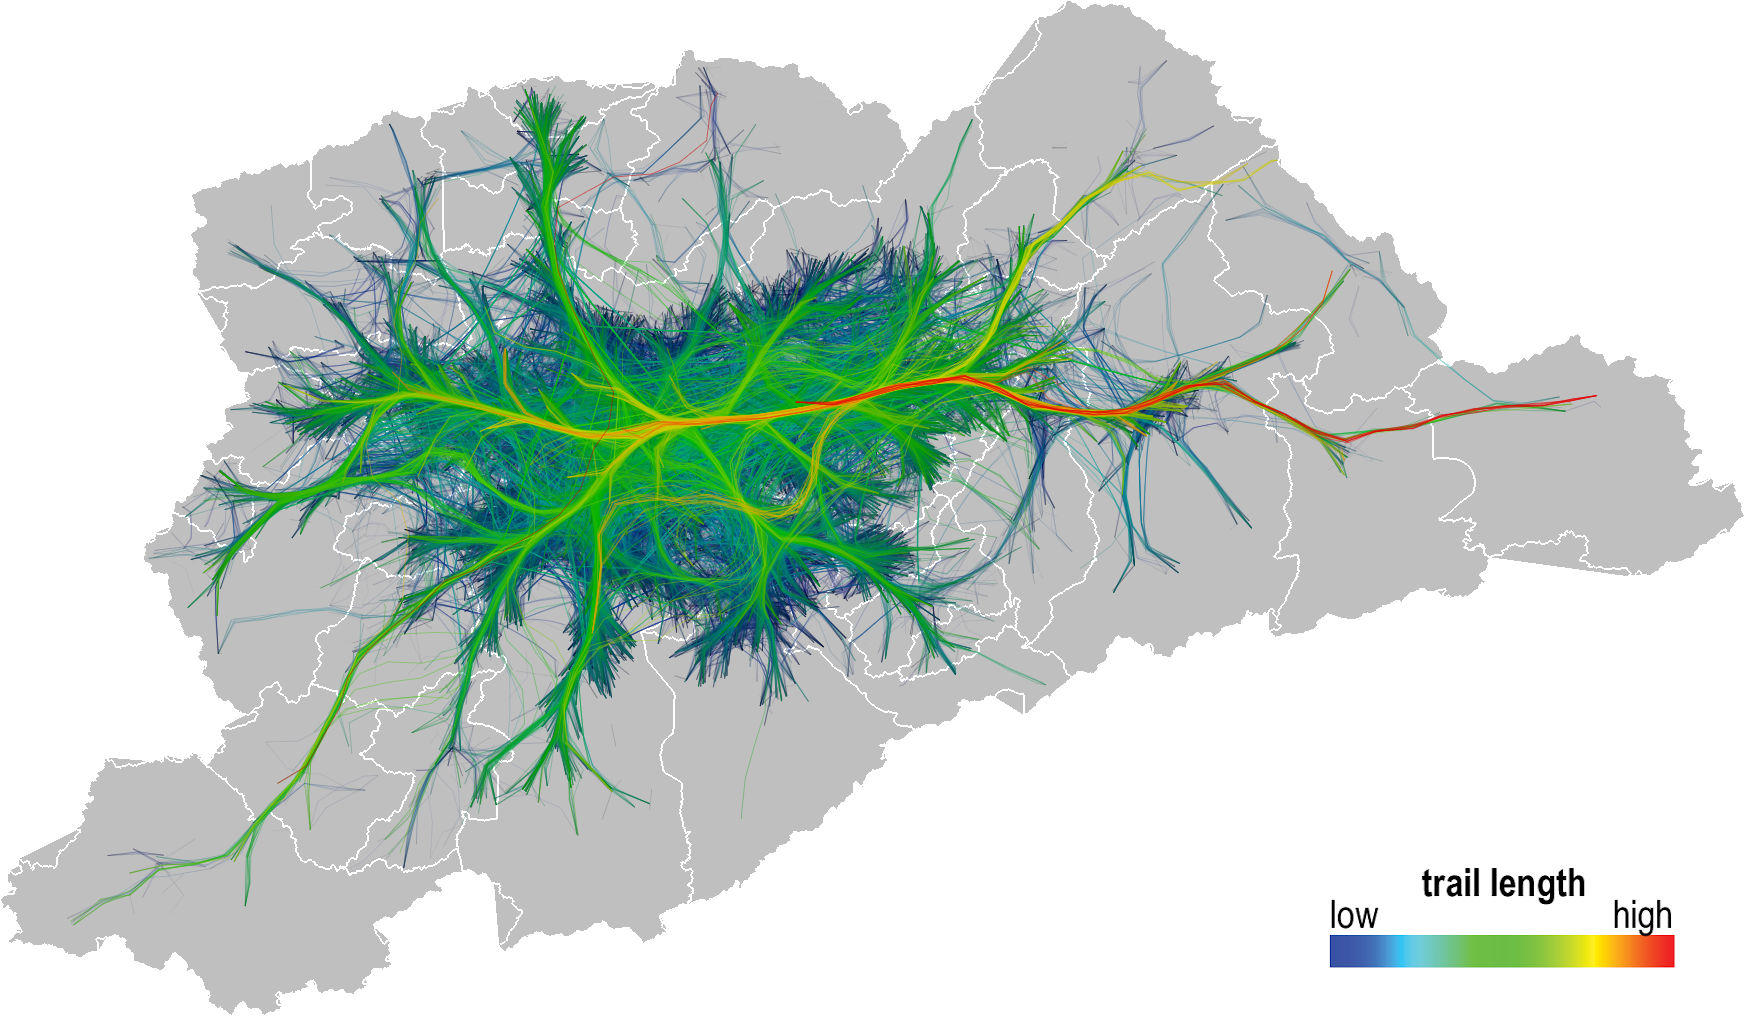
\includegraphics[width=0.98\textwidth]{figures/reason-work-leg.png}
% \caption{Distance of trips for work reasons.\label{fig:reason-work}}
% \end{figure}
  
% \begin{figure}[!htb]
% \centering
% \captionsetup{justification=centering}
% 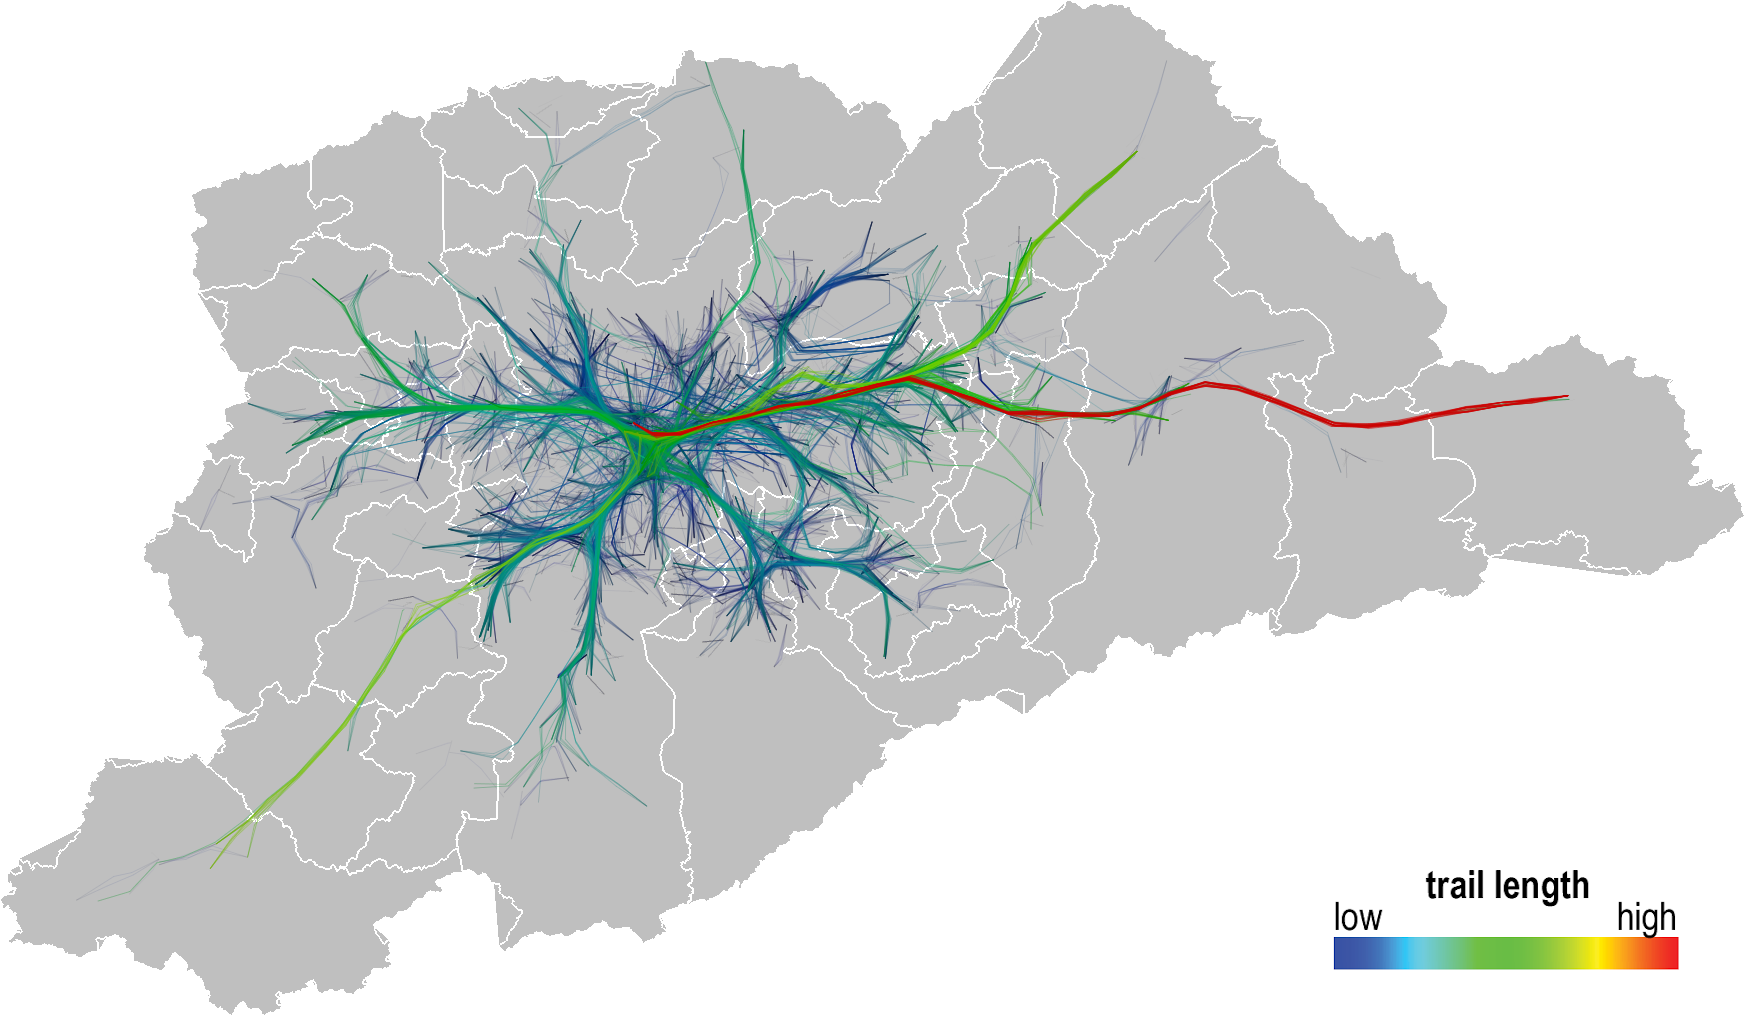
\includegraphics[width=0.98\textwidth]{figures/reason-health-leg.png}
% \caption{Distance of trips for health-related reasons.\label{fig:reason-health}}
% \end{figure}

% \begin{figure}[!htb]
% \centering
% \captionsetup{justification=centering}
% 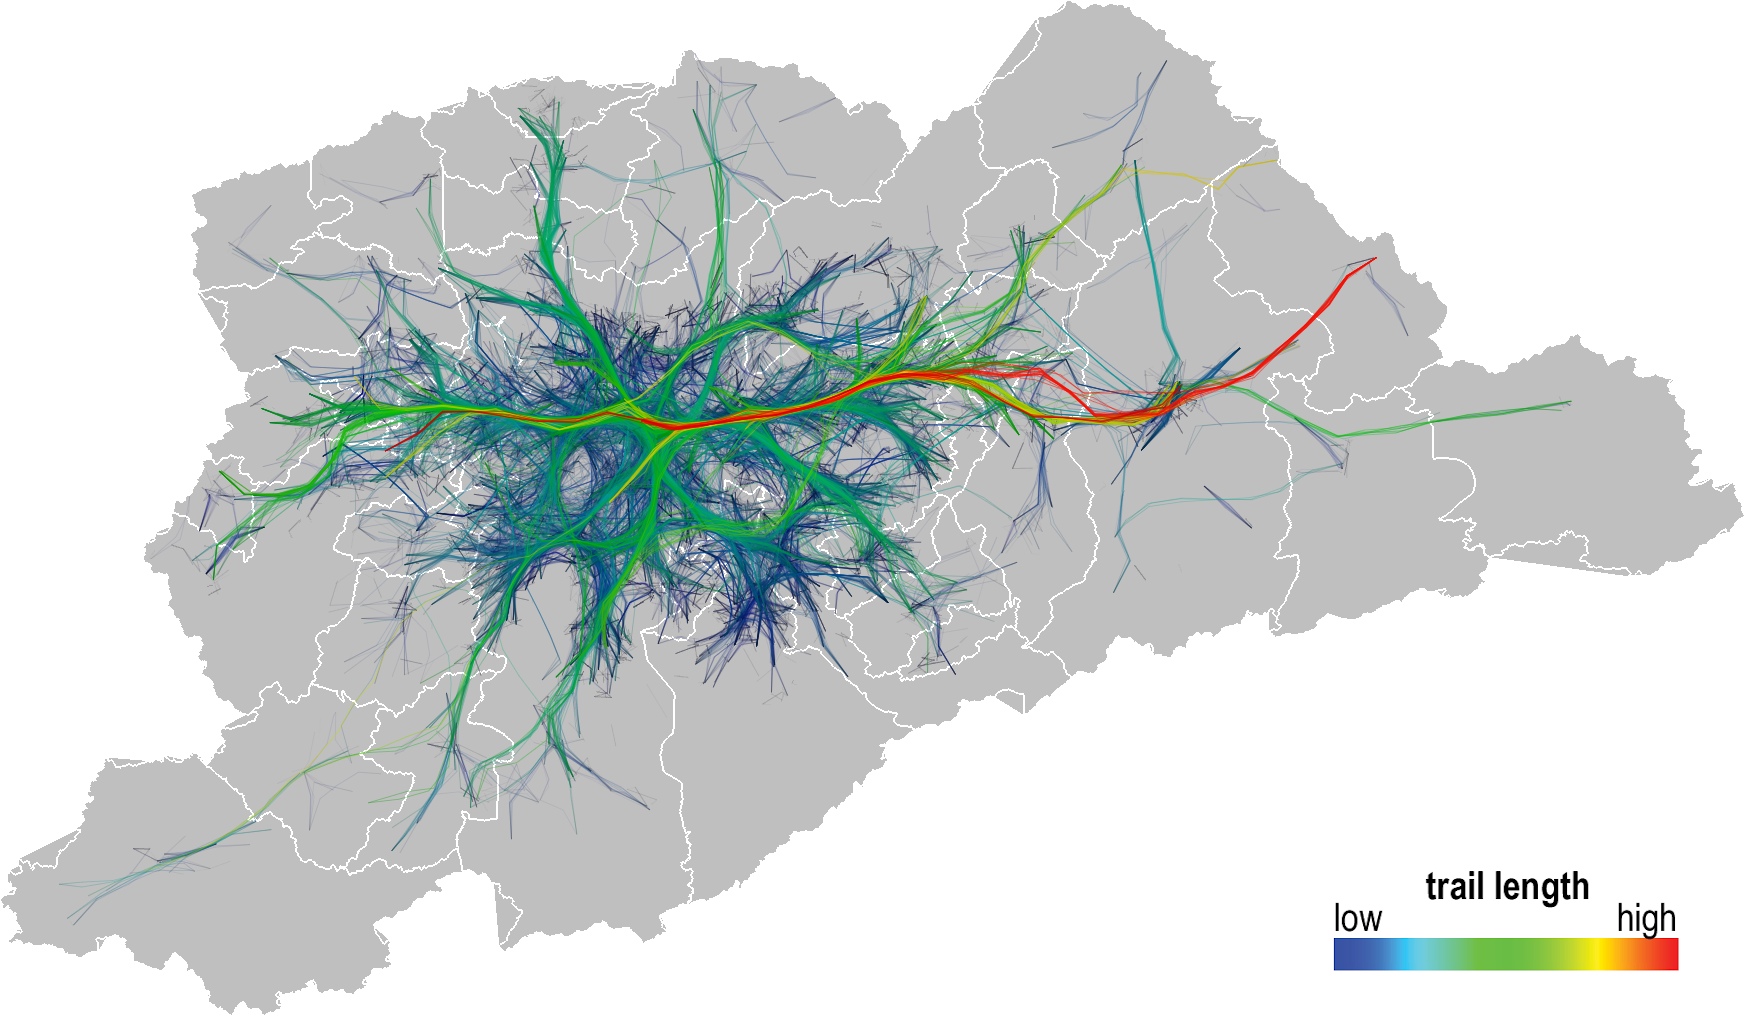
\includegraphics[width=0.98\textwidth]{figures/reason-school-leg.png}
% \caption{Distance of trips for education reasons.\label{fig:reason-education}}
% \end{figure}

% \begin{figure}[!htb]
% \centering
% \captionsetup{justification=centering}
% 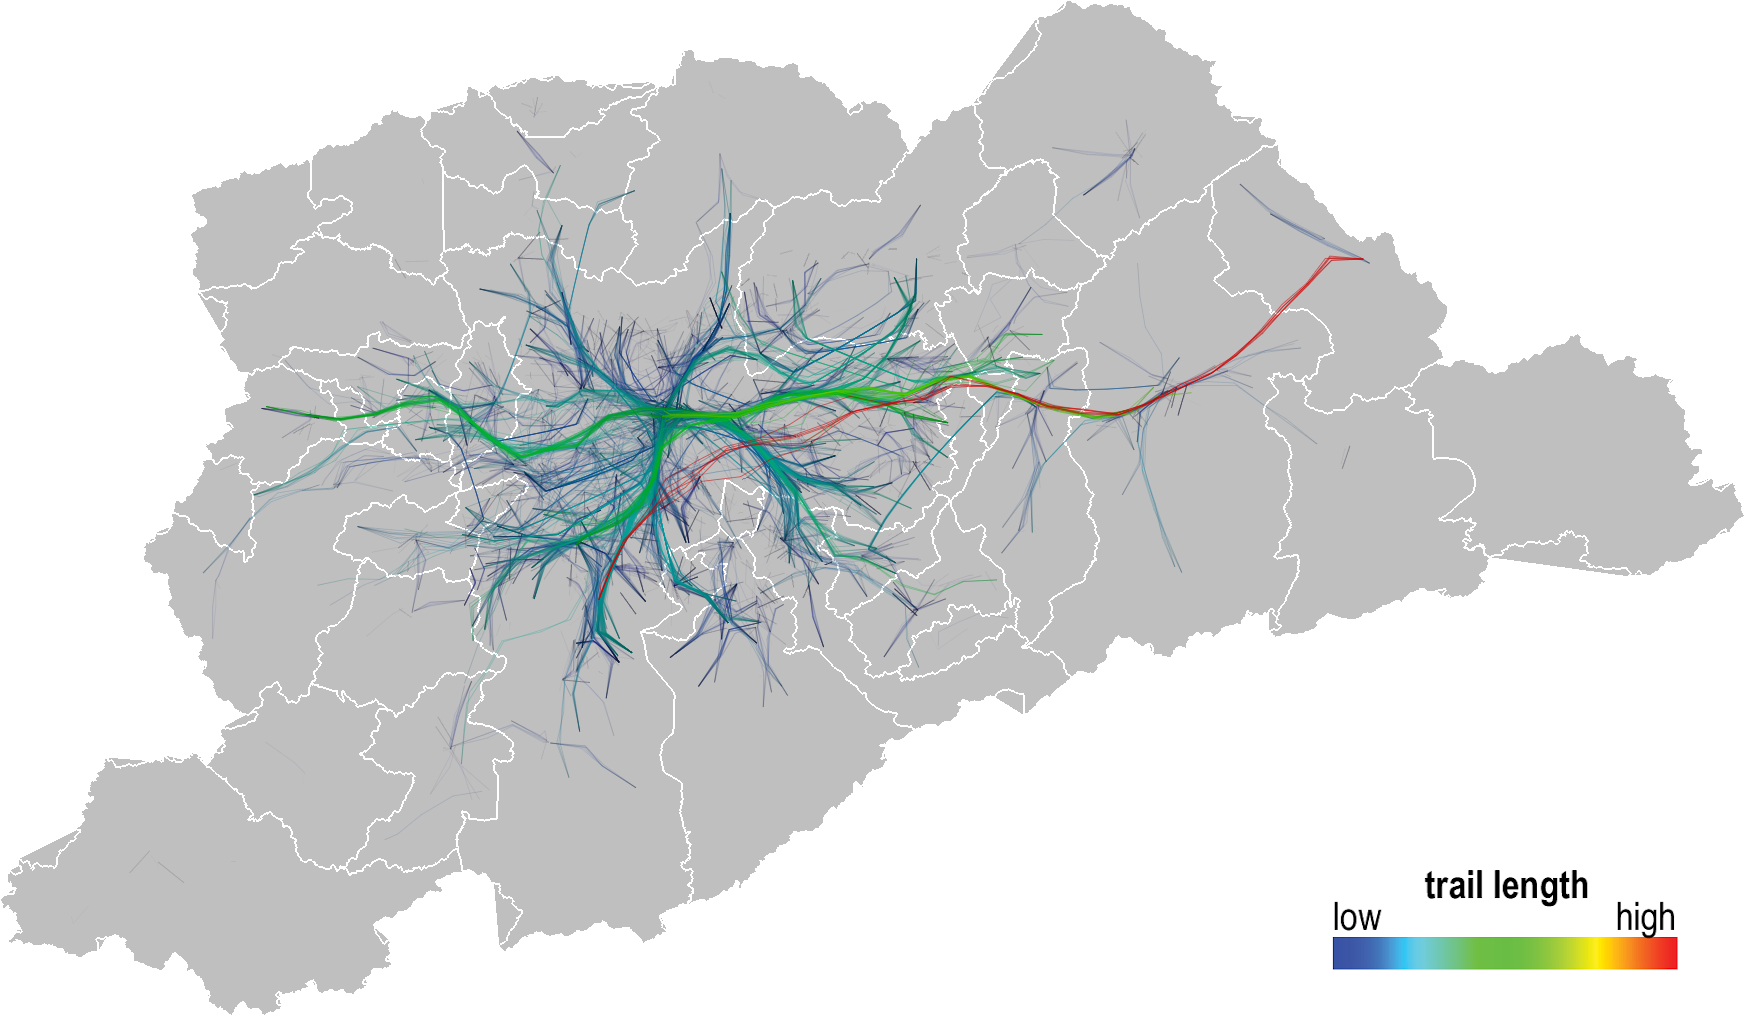
\includegraphics[width=0.98\textwidth]{figures/reason-shopping-leg.png}
% \caption{Distance of trips for shopping reasons.\label{fig:reason-shopping}}
% \end{figure}

